% !TeX program = pdflatex
% Build: pdflatex, run until the cross-references converge (two passes are
% not enough, three are needed).
%
% English edition of version 3 (revision of 24 September 2026). It mirrors
% paper_ru.tex section by section: the same \label keys, equations,
% numerical values and \cite keys, in the same order. Like paper_en_v1.tex, it
% carries no GOST R 7.0.7-2021 apparatus (article type, UDC index, bilingual
% captions, second reference list, "Information about the author" block);
% instead it follows the layout expected by international journals:
% single-language captions, a Declarations block, and one reference list with
% DOIs. All numbers are those of paper_ru.tex (analysis_v2.py with a fixed
% seed, tags [S0]-[S12]; stopping_rules.py, lpw_second_order.py,
% frontiers.py and cb_empirical.py, tags [S13]-[S22], output in
% results_v3.txt).
%
% Version 3.1 (revision of 30 September 2026, after the editorial report and
% three referee reports) mirrors the same changes of paper_ru.tex: the exposure
% of the second-order term is SUMMED OVER THE PRIMES (lpw_prime_sum.py,
% tags [S26]-[S28]); additional robustness checks (robust_extra.py, [S29]);
% base 18, the independence remark, the caption of Figure 4, the null law of
% sec:sameerror, power thresholds for a deficit, the GIMPS frontier after
% 4 September 2026.
%
% Version 3.2 (revision of 1 October 2026, after the editor's decision of major
% revision) mirrors paper_ru.tex: conditional framing of the abstract, of items 4-5
% of the contributions and of the conclusions; the m-family (M-Bm)/S, Table
% tab:mfamily; partial violations of (A1) in Table tab:stop; Remark rem:weaker
% (actual versus published frontier);
% asynchronous frontiers as lower bounds; Poisson-binomial law; Garwood-mixture
% interval; sensitivity to gaps; PRP status; attribution in tab:verify; the
% double-check protocol (revision_v32.py, tag [S30]; stopping_rules.py, [S13]).
\documentclass[11pt,a4paper]{article}

% cmap MUST precede fontenc: it embeds ToUnicode tables in the PDF, without
% which the ff/fi/fl ligatures cannot be extracted -- the text is then neither
% searchable nor correctly indexed by Crossref, Google Scholar and the like.
\usepackage{cmap}
\usepackage[T1]{fontenc}
\usepackage[utf8]{inputenc}
\usepackage[english]{babel}
\usepackage{amsmath,amssymb,amsthm}
\usepackage{booktabs}
\usepackage{graphicx}
% Figures are generated by analysis_v2.py; the English-labelled set lives in
% figs_v2/en/, the Russian one in figs_v2/ (figs/ holds the version-1 figures).
\graphicspath{{figs_v2/en/}}
\usepackage[margin=25mm]{geometry}
% xurl BEFORE hyperref: it allows long URLs to break anywhere. Without it,
% links such as t5k.org/mersenne/heuristic.html run into the right margin.
\usepackage{xurl}
\usepackage[colorlinks=true,allcolors=blue]{hyperref}
\emergencystretch=3em
\usepackage{xcolor}
\usepackage[expansion=false]{microtype}
\usepackage{caption}
\captionsetup{labelsep=period}

% Marker for quantities that cannot be obtained from the triples
% (N_b, n_min, n_max) and need the full index lists. All such markers were
% closed in version 3; the command is kept so that a stray marker still
% compiles (and shows up in red).
\newcommand{\recompute}[1]{\textcolor{red}{[recompute: #1]}}

\theoremstyle{plain}
\newtheorem{proposition}{Proposition}
\newtheorem{corollary}{Corollary}
\theoremstyle{remark}
\newtheorem{remark}{Remark}

\newcommand{\Rb}{R_b}
\newcommand{\eg}{e^{\gamma}}
\newcommand{\emg}{e^{-\gamma}}
\DeclareMathOperator{\Gam}{Gamma}
\DeclareMathOperator{\Pois}{Poisson}

\title{The observation scheme in the statistics of generalized\\
repunit primes: an exact conditional test of the\\
Lenstra--Pomerance--Wagstaff constant}
\author{Timofei S. Dokuchaev\thanks{Independent researcher, Irkutsk, Russia.
E-mail: \texttt{timofei93@yandex.ru}. ORCID:
\url{https://orcid.org/0009-0006-0510-5225}.}}
% Fixed date: \today would change on every rebuild.
\date{1 October 2026}

\begin{document}
\maketitle

\begin{abstract}
\noindent The Lenstra--Pomerance--Wagstaff (LPW) heuristic predicts
$\#\{n\le x: (b^n-1)/(b-1)\ \text{prime}\}\sim(e^{\gamma}/\ln b)\ln x$, tested
since 1993 via a ``normalized occurrence frequency''. Censoring does
not bias this frequency: the endpoint form and the OLS
slope are unbiased. The real defect: forms of the estimator disagree by up to
$29.5\%$.

We pool $B=15$ bases ($M=218$ events). The search frontiers are not
recorded; they are Neyman--Scott nuisance parameters, and the profile estimator
$M/S$ is inconsistent. If the frontier ignored the finds
(condition (A1)), the position $D_b$ of the last find is sufficient for the
frontier, and conditionally on it $N_b-1\sim\Pois(\lambda_bD_b)$ exactly. This
gives $(M-B)/S=1.838$, exact $95\%$ interval $[1.59,\,2.11]$, $p=0.67$ against
$e^{\gamma}\approx1.781$; the old test rejects a true hypothesis in $11$--$17\%$
of cases. Under (A1) the ten-percent excess over LPW comes mainly from the
observation scheme. Without (A1), agreement with LPW persists for any mean gap between the last find
and the frontier from $0$ to $3.2$ mean spacings ($2.8$ at second
order).

LPW at finite $n$ is tested via the heuristic's second-order term:
$R_b(p)$ is prime with probability $e^{\gamma}\ln(a_bp)/(p\ln b)$. Measuring
$c_b=\langle\ln a_b\rangle$ from the divisibility of $R_b(p)$ and
summing over the primes, under (A1) we obtain $1.78$ ($1.66$--$1.78$ at every truncation,
$p\ge0.598$), explaining the ``slow convergence from below''. The
homogeneity test ($p=0.935$) detects only spreads of $\kappa_b$ with coefficient
of variation above $0.37$.
\end{abstract}

\medskip
\noindent\textbf{Keywords:} repunit primes, generalized repunits, Mersenne
primes, Lenstra--Pomerance--Wagstaff conjecture, Euler--Mascheroni constant,
observation scheme, Type-I censoring, Poisson point process,
conditional likelihood, nuisance parameters, Neyman--Scott problem, sufficient
statistic, estimator bias, statistical power, computational number theory

\medskip
\noindent\textbf{Mathematics Subject Classification (2020):}
Primary 11Y11; Secondary 11N05, 62F03, 62B05, 62N01, 60G55, 11N80.

\section{Introduction}

For an integer base $b\ge2$ the generalized repunit is
\begin{equation}\label{eq:Rb}
\Rb(n)=\frac{b^{n}-1}{b-1},
\end{equation}
and $\Rb(n)$ can be prime only when $n$ is prime. For $b=2$ these are the
Mersenne numbers $M_p=2^{p}-1$. Building on the heuristics of
Wagstaff~\cite{wagstaff1983} and Pomerance~\cite{pomerance1981}, the LPW
conjecture asserts that
\begin{equation}\label{eq:LPW}
\pi_b(x)=\#\{n\le x:\ \Rb(n)\ \text{prime}\}\ \sim\ \frac{\eg}{\ln b}\,\ln x,
\end{equation}
where $\gamma$ is the Euler--Mascheroni constant; a detailed derivation of the
heuristic for $b=2$ is given in the PrimePages reference~\cite{t5k}. The base
enters~\eqref{eq:LPW} only through the factor $1/\ln b$: the constant
$\eg\approx1.7811$ is declared universal. Dubner~\cite{dubner1993} proposed
testing this universality empirically across bases, and
Bourdelais~\cite{bourdelais2009} has since maintained running estimates of the
normalized frequency, publishing them in the comments on OEIS
entries~\cite{oeis}. Related questions for the Mersenne sequence alone were
discussed recently in~\cite{wagstaff2025}. Close in spirit is
also~\cite{dominguez2026}, which looks for secondary structure in the Mersenne
exponents related to the factorization of $p-1$; methodologically it is built
like our~\S\ref{sec:struct}---stratified conditional likelihood plus a
significance test---but it tests for structure \emph{within} a single base,
whereas we test for it \emph{between} bases.

An interpretive folklore has grown up around these estimates. Base~13 is
described as ``lucky'' and base~7 as ``the unluckiest''; it is noted that the
normalized frequencies lie below the conjectured limit $\emg\approx0.5615$ and
converge to it slowly from below. The present work examines these claims, but
arrives at conclusions other than those one would naturally expect.

\subsection{Contributions}

\begin{enumerate}
\item\textbf{The frequency estimator in common use is not biased.} The scheme
in which the fitting interval ends at the largest known index does indeed
condition the estimate on the last observation being an event, and the
sufficient statistic is distributed as $\Gam(N,\lambda_b)$
(Proposition~\ref{prop:gamma}). But this does \emph{not} imply that the
normalized frequency is biased: both the endpoint form $D/(N\ln b)$ and the OLS
slope are exactly unbiased under scheme~A, and unbiased up to the factor
$1-(1+\mu)e^{-\mu}$ under scheme~B (Proposition~\ref{prop:unbiased},
Table~\ref{tab:mc}); the plug-in $\mu\approx N_b\ge7$ puts the deficit at
$0.73\%$ for the endpoint form and $2.3\%$ for OLS without the origin (an
estimate, not a bound: at the lower $95\%$ bound $\mu=3.29$ for $N_b=7$ the
deficit is $16.0\%$).
Only the reciprocal $\hat\kappa=1/\hat G$ is biased, by the factor $N/(N-1)$
(under scheme~A; under scheme~B its expectation is infinite), and that is
Jensen's inequality, not censoring. Unbiased estimators of $\kappa$
and of $1/\kappa$ cannot be reciprocals of one another; any ``correction'' that
repairs one of them damages the other (\S\ref{sec:notbias}).

\item\textbf{The genuine defect is instability with respect to the form of the
estimator.} Several numerically distinct variants are in circulation. On
identical data they disagree by as much as $29.5\%$ (base~18)---$1.7$ times the
median deviation of the estimates from $\emg$ ($17.6\%$), which is what gets
interpreted substantively; for two of the fifteen bases the choice of form
weighs more than their entire deviation from the LPW prediction. Under the
endpoint form base~18 is the third ``unluckiest'' of fifteen, and under OLS it
is the tenth, below the median. The label describes the choice of estimator, not
a property of the primes (\S\ref{sec:instability}). The size of the discrepancy
for base~18, however, is created by a single anomalous gap after an origin
$n_{\min}=2$ fixed by arithmetic.

\item\textbf{Main result: an exact conditional likelihood for scheme~B.} The
pivot $\kappa S\sim\Gam(M,1)$ is exact under the scheme ``observe until the
$N$-th event'', where $N$ is fixed by design. The data, however, arise from a
fixed frontier: the search covered $(t_0,\ln L_b]$ and the number of finds is
random. The unrecorded window widths $W_b$ are nuisance parameters whose number
grows with the number of bases; their joint MLE $\hat W_b=D_b$ leads to the
inconsistent profile estimator $M/S$---precisely the Neyman--Scott
situation~\cite{neymanscott1948}. We show (Proposition~\ref{prop:cond}) that
$D_b$ is sufficient for $W_b$ when $\kappa$ is held fixed and that,
conditionally on $D_b$, the quantity $N_b-1$ is $\Pois(\lambda_bD_b)$, with
\emph{the window width $W_b$ not entering this distribution}. Hence
$M-B\mid D\sim\Pois(\kappa S)$ is an exact Poisson pivot, and $(M-B)/S$ is the
conditional maximum-likelihood estimator in the sense of
Andersen~\cite{andersen1970}, exactly conditionally unbiased; it is also
obtained by integrating over $W_b$ against the measure $dW_b$
(Remark~\ref{rem:integrated}). No moment approximations, no exponentially small
remainders and no simulation-based inversion of intervals are required
(\S\ref{sec:scheme}). Exactness refers to the Poisson model~\eqref{eq:lam}: if
the heuristic is read literally, as Bernoulli trials at the prime indices, the
conditional law is Poisson-binomial and the Poisson intervals are conservative or
practically exact (\S\ref{sec:second}). The distinction between the schemes is itself classical,
and the unbiasedness of $(N-1)/D$ under scheme~A and the loss of one observation
per stratum are textbook facts; we lay no claim to them. What is new is the
setting: the frontier is \emph{undocumented}, so the exposure must be
reconstructed from the finds themselves, and the correction turns out to be
proportional to the number of bases (Remark~\ref{rem:priority}).

\item\textbf{Numerical consequence and its condition.} Under (A1) the exact
conditional inference gives $\hat\kappa=1.838$ with a $95\%$ interval
$[1.594,\,2.109]$ and $p=0.672$: the excess over LPW shrinks from $10.3\%$ to a
statistically insignificant $3.2\%$. Under scheme~B the old Gamma pivot rejects a
true hypothesis in $11$--$17\%$ of cases (\S\ref{sec:calib}); the spread depends on
how far the frontier has advanced, which is precisely why it is reported as a
range. Without (A1) the stopping rule enters the inference through a single
number---the mean gap $m$ between the last find and the frontier in units of the
mean spacing: by Wald's identity $(M-Bm)/S$ is unbiased in the sense of
expectations, and with $m$ known the shifted Poisson test approximately keeps its
level ($0.043$--$0.056$) under every stopping rule considered, partial violations of
(A1) included (Table~\ref{tab:stop}). The conclusion ``LPW is not rejected'' is
robust: it holds for every $m$ from $0$ (stopping exactly at a find) to $3.2$, and
to $2.8$ with the second-order term (Table~\ref{tab:mfamily}); this covers drought
$g=2$ as well ($\bar m=2.14$). LPW is not rejected from above for any
$m\ge0$; it would be rejected from below only for a mean gap exceeding $3.2$
($2.8$) mean spacings. Only the residual
excess depends on $m$: $10.8\%$ at $m=0$, $3.2\%$ under (A1), and zero at
$m=1.42$.

\item\textbf{Key assumption about the frontiers and its cost.} Besides the
Poisson model and contiguous coverage of the search (\S\ref{sec:data}), the
conclusion that the excess is created by the observation scheme rests on
condition (A1): the frontier was chosen without regard to the finds (the
condition concerns the actual search horizon, not the published bound;
Remark~\ref{rem:weaker}). The estimators $(M-1)/S$ and
$(M-B)/S$ are built on the same statistics $(N_b,D_b)$ and differ by $6.9\%$;
which of them is right is determined not by the data but by how the data were
collected. Without (A1) only an \emph{upper} bound in the sense of expectations
holds rigorously: by Wald's identity $\mathbb E[M]\ge\kappa\,\mathbb E[S]$ under
any stopping rule. There is no lower bound: the rule ``stop the search after a
long stretch without finds'' biases even $(M-B)/S$ upward
(Remark~\ref{rem:bracket}, Table~\ref{tab:stop}); it cannot produce a rejection
of LPW from above: the true $\kappa$ is then lower still, and a rejection from below
would require a very long drought (\S\ref{sec:pooled}). An attempt to sidestep
the choice by assembling the estimate from per-base pieces that are unbiased by
construction fails (\S\ref{sec:noescape}). The four documented frontiers
($b=2,10,22,26$) do not settle (A1): three of them predate the data snapshot and
give only lower bounds on the gap for it, the moment of publication may itself be
tied to the finds, and the bases with a published frontier are not a random
sample. Only the $b=2$ frontier is synchronous with the snapshot, and it is
consistent with (A1) (\S\ref{sec:frontiers}). The only radical remedy is to
publish the frontiers $L_b$.

\item\textbf{Lucky bases: what the test cannot do.} Conditioning on $K=M-B$
makes the null distribution of the homogeneity test exact (multinomial), with
no appeal to $\chi^2$ asymptotics. We obtain $\Lambda=7.13$ on $14$ degrees of
freedom, exact $p=0.935$. But its power is such that it reliably resolves only
a spread of $\kappa_b$ with a coefficient of variation of order $0.37$ or more
(\S\ref{sec:homog}). The correct conclusion is
``base-dependent frequencies are not required by the data'', not ``they do not
exist''.

\item\textbf{The second-order term of the heuristic itself.} At finite $n$ the
LPW heuristic predicts not a constant intensity but
$\lambda_b(t)=(\kappa/\ln b)(1+c_b/t)$: the divisors of $\Rb(p)$ are at least
$2p+1$. The exact conditional inference carries over to this model in closed
form (\S\ref{sec:second}), but the exposure must be summed over the prime indices
rather than integrated with density $1/\ln n$: for origins $n_{\min}=2$--$19$ the
integral overstates it by $1.04$ in $t$ per base on average (the constant $E$ of
Mertens' first theorem) and understates the estimate by $9.0\%$ on the full
sample. The positions of the finds determine $c_b$ only weakly, so
we measure it directly from the divisibility of $\Rb(p)$: $c_b=0.43$--$1.11$,
with mean $0.67$, stable with respect to the threshold; Wagstaff's device gives
values twice as large. These values are predicted from first principles---from
the primality of the numbers $2kp+1$ and the quadratic character of $b$
(correlation $0.976$)---so that $c_b$ depends only on the squarefree part of
$b$. The method has been validated on data generated by the heuristic itself at
the level of prime indices: it is unbiased and attains nominal coverage, whereas
the constant-intensity model overstates $\kappa$ by $3$--$8\%$. With the
calibrated $c_b$ the estimate of $\kappa$ drops by $3.2\%$ on the full sample and
by $5.0$--$5.8\%$ under truncation, that is, comparably to the cost of the
choice of observation scheme. Under (A1), at every lower truncation level one
obtains
$\hat\kappa\approx1.66$--$1.78$, LPW is not rejected ($p\ge0.598$), and the
same term explains the folklore ``slow convergence from below''.

\item\textbf{An explicit power calculation.} With a two-sided test the pooled
sample resolves an excess over $\eg$ of at least $21.3\%$ and a deficit of at
least $19.2\%$; the Mersenne sequence alone, $45.5\%$ and $37.4\%$ respectively
(\S\ref{sec:power}). The test convention is
stated explicitly, since the one-sided variant gives a noticeably different
threshold ($18.7\%$).
\end{enumerate}

Section~\ref{sec:sameerror} works through a narrower but instructive episode: a
naive regression of the Mersenne counting function produces an apparently
significant negative intercept, which turns out to be an artifact of
conditioning. We include it as a worked example of the same error in a different
guise.

\section{Model and data}\label{sec:data}

\subsection{The Poisson model}
Put $t=\ln n$. To leading order the heuristic~\eqref{eq:LPW} leads to a model in
which the indices of generalized repunit primes to base~$b$ form a homogeneous
Poisson point process on the $t$-axis with constant intensity
\begin{equation}\label{eq:lam}
\lambda_b=\frac{\kappa}{\ln b},\qquad \text{LPW:}\ \ \kappa=\eg=1.781072\ldots
\end{equation}
Universality is the assertion that a single parameter $\kappa$ governs all
bases. The form $\kappa/\ln b$ with a common $\kappa$ follows from the structure
of the divisors of $\Rb(p)$. Let $p$ be an odd prime with $p\nmid b-1$. If a prime
$q\nmid b-1$ divides $\Rb(p)$, then $b$ has order $p$ modulo~$q$, whence
$q\equiv1\pmod p$, and since $\Rb(p)$ is odd, $q\equiv1\pmod{2p}$; and if
$q\mid b-1$, then $\Rb(p)\equiv p\not\equiv0\pmod q$. Hence no prime $q<2p+1$
divides $\Rb(p)$ for any such~$b$: $\Rb(p)$ has no base-dependent local factors at leading
order, of the kind of a Bateman--Horn singular series, and the gain
$\eg\ln(2p)$ from the absence of small divisors is the same for all bases
(\S\ref{sec:second}). The base enters the leading term only through the size of
the number, that is, through $1/\ln b$; dependence on $b$ appears only at second
order, through the symbol $(b/q)$ for $q=2kp+1$, and is accounted for
in~\S\ref{sec:second}. The Poisson idealization rests on the Cram\'er model of
independent trials and on pairwise coprimality:
$\gcd\bigl(\Rb(p),\Rb(p')\bigr)=\Rb\bigl(\gcd(p,p')\bigr)=1$ for distinct primes
$p,p'$. It is a working assumption, not a theorem: even for the ordinary primes
the Poisson law in short intervals has been derived only conditionally, from the
Hardy--Littlewood conjectures~\cite{gallagher1976}; on scales $(\ln x)^{A}$, $A>1$,
the Cram\'er model is known to fail~\cite{maier1985}; and refinements of the
Poisson picture in short intervals remain conjectural~\cite{jha2026}. At finite
$n$ the heuristic itself specifies not a homogeneous Poisson process but
Bernoulli trials at the prime indices with a slowly varying probability; this is
accounted for in~\S\ref{sec:second}. We adopt~\eqref{eq:lam}
as a model and treat $\kappa$ throughout as a quantity to be estimated; this
reduces the question ``is LPW true?'' to a one-parameter one and makes the bases
poolable. The word ``exact'' in this paper refers to inference in
model~\eqref{eq:lam} and its inhomogeneous generalization: in the Bernoulli-trial
model the conditional law of the number of events is Poisson-binomial rather than
Poisson, and the Poisson intervals are conservative or practically exact
(\S\ref{sec:second}, Remark~\ref{rem:indep}).

\subsection{Admissible bases}\label{sec:bases}
Bases that are perfect powers are excluded: for $b=c^{m}$ with $m>1$ and a prime
$n\nmid m$ the number $R_c(n)>1$ divides $\Rb(n)$, so there are only finitely many
primes $\Rb(n)$ (the index $n$ must divide $m$), and there is no process of finds
at all. Bases $4,8,9,16$ are therefore omitted. For prime $n$ the bases $b\le26$
have no other infinite algebraic families: for prime $n$ we have
$\Rb(n)=\Phi_n(b)$, and of the known algebraic factorizations of a cyclotomic
polynomial at a $b$ that is not a perfect power only the Aurifeuillean one, at
$n=s$, applies (see below). The arithmetic of small indices has a few further finite
effects. We note separately one \emph{infinite arithmetic} family of forced
composites: if $q=2p+1$ is prime, $q\nmid b-1$ (which certainly holds when
$2p+1\ge b$) and $(b/q)=+1$, then $q\mid\Rb(p)$ (the
generalization of the Euler--Lagrange theorem for $M_p$ with $p\equiv3\pmod4$),
and $\Rb(p)$ is composite except when $\Rb(p)=q$ ($b=2$, $p=3$).
It acts at every $p$ with density of order $1/\ln p$ and is not excluded but
enters the second-order term (\S\ref{sec:second}, the case $k=1$
in~\eqref{eq:cbth}). If $p\mid b-1$, then $\Rb(p)\equiv p\pmod{b-1}$ is divisible
by~$p$ and hence composite. If $p=s$, where $s\equiv1\pmod4$ is the squarefree
part of $b$, the Aurifeuillean factorization applies ($b=5,13,17,20$). Finally,
$\Rb(2)=b+1$ is prime exactly for $b=2,6,10,12,18$, so for these five bases the
origin $n_{\min}=2$ is fixed by arithmetic, not by chance. In the main set all
these finite effects concern only $n\le19$; their influence is examined in~\S\ref{sec:robust} and
accounted for in~\S\ref{sec:second}. Within the declared range
the selection does not depend on the results: we take \emph{all} bases
$2\le b\le20$ that are not perfect powers, which gives $B=15$; no base was
excluded or added on the strength of its estimate. Each of them has at least
eight known indices (the minimum is attained at $b=18$: eight terms of A133857).

We stress, however, that the upper limit $b\le20$ is itself a conventional round
number and not a consequence of the criterion ``at least eight indices'': that
criterion continues to hold beyond it (A127996 for $b=21$ has eight terms,
A127997 for $b=22$ has nine) and first fails at $b=23$ (A204940, six terms). To
make sure the limit does not look chosen after the fact, we tested its influence
directly. Extending the set to all bases $b\le26$ that are not perfect powers
(this adds $b=21,22,23,24,26$; $b=25=5^2$ is excluded algebraically; for $b=22$
the origin $n_{\min}=2$ is also fixed by arithmetic, $R_{22}(2)=23$, and for
$b=24$ the condition $p\mid b-1$ makes $R_{24}(23)$ composite, that is, it
concerns the index $23>19$) gives $B=20$, $M=253$ and
\[
  \frac{M-1}{S}=1.9776,\qquad \frac{M-B}{S}=1.8285,
\]
that is, it shifts the main estimate~\eqref{eq:resB} by $0.5\%$---more than an
order of magnitude less than the price of the choice of observation scheme
(\S\ref{sec:scheme}). The homogeneity test on the extended set does not reject
homogeneity ($\Lambda=10.24$ on $19$ degrees of freedom, exact $p=0.953$;
tag~[S17]). No conclusion of this work depends on the limit $b\le20$; we retain
it as pre-declared.

\begin{remark}[Selection on the number of finds]\label{rem:selection}
Formally the limit $b\le20$ was declared in advance, but it was chosen in a
world where the numbers of known terms had already been published, and the size
of the threat should be stated. The conditional inference of \S\ref{sec:scheme}
conditions on $N_b\ge1$---which is harmless: under scheme~B with the frontier
$W_b=N_b/\lambda_b$ the bias of $(M-B)/S$ is $+0.04\%$. Were a base admitted only
with $N_b\ge7$, the estimate would be biased \emph{upward} by $3.1\%$ (tag~[S30]),
that is, by an amount of the same order as the residual excess of $3.2\%$. What
protects the conclusion from such selection is not the sign of any shift but the
fact that the rule $b\le20$ does not depend on the number of finds, together with
a direct check: lifting the limit to $b\le26$ adds, in particular, the base
$b=23$ with six terms and shifts the estimate \emph{downward}, from $1.8381$ to
$1.8285$---in the direction predicted by selection on the number of finds, and by
an order of magnitude less than the price of the observation scheme.
\end{remark}

\subsection{The data and their status}
Table~\ref{tab:data} lists the sequences used, retrieved on 27 August 2026
(cross-check: Appendix~\ref{app:data}). Four caveats matter.

\paragraph{Probable primes.} For large indices most of the entries are probable
primes established by a Fermat or strong Fermat test after trial division. PRP
status begins far below one million: according to the OEIS entries, from
$18\,743$ for $b=13$ (A016054), from $19\,697$ for $b=14$ (A006032), after
$57\,917$ for $b=3$ (A028491), from $201\,359$ for $b=5$ (A004061). The count is
biased upward only if a Fermat pseudoprime has been mistaken for a prime, which
for numbers of this size is practically unheard of; the opposite risk, a missed
find (below), is more real. Sensitivity to both is examined
in~\S\ref{sec:robust}.

\paragraph{Verification frontiers.} For $b=2$ the GIMPS project~\cite{gimps}
publishes two frontiers: all exponents below $X_{\mathrm{ver}}=81\,648\,221$
have been tested twice, which gives exactly $50$ Mersenne primes, whereas all
exponents below $X_{\mathrm{ft}}=141\,308\,443$ have been tested at least once,
which gives $52$. The two largest exponents are provisional: unverified
candidates remain between them. The analysis of~\S\ref{sec:sameerror}, where the
frontier is used explicitly, is restricted to the $50$ verified exponents. The
pooled analysis is insensitive to this choice (\S\ref{sec:robust}).

Both frontiers are moving quantities, so we fix the moment of reading: the
PrimeNet Milestones report, 27 August 2026. No conclusion depends on the exact
value of $X_{\mathrm{ver}}$: it suffices that it lies between
$M_{50}=77\,232\,917$ and $M_{51}=82\,589\,933$, and this holds for every value
the report has taken from the start of 2026 to 4 September 2026. Once
double-checking below $M_{51}$ was complete the frontier moved past it
($83\,200\,483$ on 30 September 2026); the slice of double-checked exponents then
includes $M_{51}$ as well, but the computations of~\S\ref{sec:sameerror} use the
snapshot of 27 August 2026, and the pooled analysis does not depend on this slice.

\paragraph{The status of entry A000043.} On the retrieval date (27 August 2026)
the DATA section of that entry contained $50$ terms and stopped at
$77\,232\,917$: OEIS regards the order of the subsequent exponents as unproven
until double-checking is complete. The exponents $82\,589\,933$ and
$136\,279\,841$ are known and documented by GIMPS (and are mentioned in the
comments on A000043), but formally they were not part of DATA. After
double-checking below $82\,589\,933$ was completed (GIMPS report of 4 September
2026), that exponent was added to DATA as the $51$st term (checked on
24 September 2026); this does not affect the computations, since it is already
included. We include both
exponents, because the statistic~\eqref{eq:pivotB} uses only the position
of the last event and not its ordinal number; \S\ref{sec:robust} verifies that
restricting base~2 to the fifty double-checked exponents does not change the
conclusion.

\paragraph{Search bounds and completeness of coverage for $b>2$.} For the other
bases a dated and attributed frontier above the last find has been published
only for $b=10$: ``Search limit is 10800000, currently'' (S.~Batalov, comment
on A004023, 1 July 2021). In the extended set it is joined by $b=22$ and $b=26$,
with the bound $10^5$ (R.~Price, comments on A127997 and A127999, 2012). For the
remaining bases the OEIS entries contain only the dates of the finds, and
participants in the distributed search state explicitly that the search limits
for most bases are unknown. It is precisely this gap that is the subject
of~\S\ref{sec:scheme} and, we believe, the principal obstacle to a quantitative
test of LPW; the four documented frontiers are used in~\S\ref{sec:frontiers}. We
note separately that the entire construction assumes that the search covered
$(t_0,\ln L_b]$ \emph{contiguously}. If the sieved ranges contain gaps---a common
occurrence in distributed searching---then $M$ is understated relative to the
exposure and $\hat\kappa$ is biased downward, that is, in the same direction as
our main conclusion. In general, completeness of coverage cannot be checked from
published data; how large such a gap would have to be to change the conclusion
is assessed in~\S\ref{sec:robust}. That such gaps are real is shown by base~$5$. In 2024 the
probable primes $R_5(4\,939\,471)$ and $R_5(5\,154\,509)$ were found
(R.~Propper); they are not in the OEIS, and summary tables mark the range
$3\,300\,593$--$4\,939\,471$ as not searched contiguously. For the conditional
inference this matters: law~\eqref{eq:condlaw} requires contiguous coverage of
$(t_0,t_0+D_b)$. We therefore retain $n_{\max}=3\,300\,593$. Including both
numbers, which is admissible only under contiguous coverage, would give
$\hat\kappa=1.852$ instead of $1.838$ (tag~[S18]). This is one more argument for
publishing not only the frontiers but also the sieving protocols.

\begin{table}[t]
\centering
\caption{Sequences used. $N_b$ is the number of events strictly to the right of
$t_0=\ln n_{\min}$, that is, one less than the number of known prime indices: the
smallest index sets the origin, not an event; $K_b=N_b-1$ is the conditional event
count entering~\eqref{eq:pivotB}. The $D_b$ column is rounded, but all computations
use exact $D_b=\ln n_{\max}-\ln n_{\min}$. In the last row $M=\sum_b N_b$, $K=M-B$
and $S=\sum_b D_b/\ln b$; the quantity $S$ is not the sum of the $D_b$ column.
Source: OEIS entries, retrieved on 27 August 2026; for $b=2$ the exponents
$82\,589\,933$ and $136\,279\,841$ are taken from GIMPS (\S\ref{sec:data}).}
\label{tab:data}
\small
\begin{tabular}{rlrrrrrrr}
\toprule
$b$ & OEIS & primes & $N_b$ & $K_b$ & $n_{\min}$ & $n_{\max}$ & $D_b$ & $D_b/\ln b$\\
\midrule
2 & A000043 & 52 & 51 & 50 & 2 & 136\,279\,841 & 18.0371 & 26.0220\\
3 & A028491 & 23 & 22 & 21 & 3 & 8\,530\,117 & 14.8605 & 13.5266\\
5 & A004061 & 19 & 18 & 17 & 3 & 3\,300\,593 & 13.9110 & 8.6434\\
6 & A004062 & 17 & 16 & 15 & 2 & 3\,360\,347 & 14.3344 & 8.0002\\
7 & A004063 & 10 & 9 & 8 & 5 & 1\,264\,699 & 12.4409 & 6.3934\\
10 & A004023 & 11 & 10 & 9 & 2 & 8\,177\,207 & 15.2237 & 6.6116\\
11 & A005808 & 13 & 12 & 11 & 17 & 1\,868\,983 & 11.6077 & 4.8408\\
12 & A004064 & 14 & 13 & 12 & 2 & 769\,543 & 12.8604 & 5.1754\\
13 & A016054 & 13 & 12 & 11 & 5 & 1\,503\,503 & 12.6139 & 4.9178\\
14 & A006032 & 11 & 10 & 9 & 3 & 1\,724\,417 & 13.2618 & 5.0252\\
15 & A006033 & 10 & 9 & 8 & 3 & 639\,833 & 12.2704 & 4.5311\\
17 & A006034 & 12 & 11 & 10 & 3 & 1\,990\,523 & 13.4053 & 4.7315\\
18 & A133857 & 8 & 7 & 6 & 2 & 1\,270\,141 & 13.3615 & 4.6228\\
19 & A006035 & 11 & 10 & 9 & 19 & 209\,359 & 9.3074 & 3.1610\\
20 & A127995 & 9 & 8 & 7 & 3 & 984\,349 & 12.7011 & 4.2397\\
\midrule
\multicolumn{3}{l}{total} & $M=218$ & $K=203$ & & & & $S=110.4423$\\
\bottomrule
\end{tabular}
\end{table}

\section{What is biased and what is not}\label{sec:notbias}

\subsection{The estimators in common use}
Dubner~\cite{dubner1993} and Bourdelais~\cite{bourdelais2009} characterize a
base~$b$ by a normalized occurrence frequency obtained by fitting a straight
line to $\ln n_k$ against $k$ and dividing by $\ln b$. By~\eqref{eq:lam} the
expected slope is $1/\lambda_b=\ln b/\kappa$, so the normalized frequency
estimates
\begin{equation}\label{eq:G}
G_b=\frac{1}{\kappa},\qquad\text{LPW:}\ \ G_b=\emg=0.5614595\ldots
\end{equation}
Several variants are in circulation---ordinary OLS with an intercept, regression
through the origin, and the endpoint form $\hat G_b=D_b/(N_b\ln b)$ with
$D_b=t_{N_b}-t_0$. All of them share one structural feature: the fitting
interval ends at the largest known index. Regression through the origin is
understood in two ways. The line through the point $(0,t_0)$, that is, OLS of
$t_k-t_0$ on $k$ without an intercept, has weights $w_k=k/\sum_jj^2$ with
$\sum_kw_kk=1$ and is unbiased under scheme~A by the same argument as
Proposition~\ref{prop:unbiased}. The line through the literal origin of the
$(k,\ln n_k)$ plane is biased: $\mathbb E[\hat\beta]=1/\lambda+3t_0/(2N+1)$, which
is from $5.2\%$ ($b=2$) to $25.4\%$ ($b=19$) of $1/\lambda$ (tag~[S30]); this
variant is not considered below.

\subsection{The exact distribution}

\begin{proposition}[Conditional law of the right endpoint]\label{prop:gamma}
Let the events form a homogeneous Poisson process of intensity $\lambda$ on
$(t_0,\infty)$, and let $t_1<\dots<t_N$ be its first $N$ events after $t_0$.
Then $D:=t_N-t_0$ has the $\Gam(N,\lambda)$ distribution with density
$\lambda^{N}d^{N-1}e^{-\lambda d}/(N-1)!$. Conditionally on $D=d$, the preceding
$N-1$ events are distributed as the order statistics of $N-1$ independent
uniform variables on $(t_0,t_0+d)$.
\end{proposition}

\begin{proof}
The waiting times $t_1-t_0,\dots,t_N-t_{N-1}$ are independent
$\mathrm{Exp}(\lambda)$ variables, and a sum of $N$ of them is
$\Gam(N,\lambda)$. The joint density of $(t_1,\dots,t_N)$ on
$t_0<t_1<\dots<t_N$ is the product of the densities of the spacings, that is,
$\lambda^Ne^{-\lambda(t_N-t_0)}$. Dividing by the $\Gam(N,\lambda)$ density at
$d=t_N-t_0$ gives the conditional density $(N-1)!/d^{\,N-1}$ of the first $N-1$
events on $t_0<t_1<\dots<t_{N-1}<t_0+d$, which is the density of the order
statistics of $N-1$ independent uniform variables.
\end{proof}

\noindent In the data $t_0=\ln n_{\min}$ is the position of the first find for
ten of the fifteen bases, and is fixed by arithmetic for five ($b=2,6,10,12,18$,
\S\ref{sec:bases}). This does no harm: the time of the first event is a stopping
time, and by the strong Markov property the process to its right is again Poisson
with the same intensity. The same applies to
Propositions~\ref{prop:unbiased}--\ref{prop:delta} and to~\eqref{eq:condinhom}.

\begin{corollary}[Bias of the reciprocal]\label{cor:kappa}
The maximum-likelihood estimator of $\lambda$ based on $D$ alone is
$\hat\lambda=N/D$, and
\begin{equation}\label{eq:bias}
\mathbb E[\hat\lambda]=N\,\mathbb E[D^{-1}]=\frac{N}{N-1}\,\lambda,
\end{equation}
since $\mathbb E[D^{-1}]=\lambda/(N-1)$ for $D\sim\Gam(N,\lambda)$ with $N\ge2$.
The estimator $\tilde\lambda=(N-1)/D$ is exactly unbiased.
\end{corollary}

\subsection{What does not follow from Corollary~\ref{cor:kappa}}

It is natural to conclude that, since $\hat\lambda$ is inflated by the factor
$N/(N-1)$, the frequency $\hat G_b$ must be deflated by the same factor. This is
false under either of the two observation schemes analyzed below.

\begin{proposition}[Unbiasedness of the frequency]\label{prop:unbiased}
\emph{(a) Scheme~A.} Under the hypotheses of Proposition~\ref{prop:gamma}:
\begin{enumerate}
\item[\rm(i)] the endpoint estimator is exactly unbiased:
$\mathbb E\!\left[\dfrac{D}{N\ln b}\right]=\dfrac{1}{\lambda\ln b}=G_b$;
\item[\rm(ii)] the OLS slope in the regression of $t_k$ on $k$ is exactly
unbiased: $\mathbb E[\hat\beta]=1/\lambda$;
\item[\rm(iii)] consequently the ``corrected'' quantity
$\tilde G_b=\frac{N}{N-1}\hat G_b$ is biased \emph{upward}, by exactly the
factor $N/(N-1)$.
\end{enumerate}
\emph{(b) Scheme~B.} Let the process be observed on a window of width $W$, and
put $\mu=\lambda W$; the estimators are set to zero where they are undefined.
Then
\begin{equation}\label{eq:BunbiasedB}
\mathbb E\!\left[\frac{D}{N}\,\mathbf 1_{\{N\ge1\}}\right]
=\mathbb E\bigl[\hat\beta_0\,\mathbf 1_{\{N\ge1\}}\bigr]
=\frac{1}{\lambda}\Bigl(1-(1+\mu)e^{-\mu}\Bigr),
\end{equation}
where $\hat\beta_0$ is the OLS slope through the points $(k,t_k)$,
$k=0,\dots,N$, \emph{including} the origin. For the slope $\hat\beta_1$ through
the points $k=1,\dots,N$ \emph{without} the origin, which is defined for
$N\ge2$,
\begin{equation}\label{eq:BunbiasedOLS}
\mathbb E\bigl[\hat\beta_1\bigm|N\ge2\bigr]
=\frac{1}{\lambda}\cdot
\frac{1-\bigl(1+\mu+\mu^2/2\bigr)e^{-\mu}}{1-(1+\mu)e^{-\mu}} .
\end{equation}
Both forms are thus unbiased up to a term exponentially small in $\mu$; at
$\mu=7$ the deficit is $0.73\%$ in~\eqref{eq:BunbiasedB} and $2.25\%$
in~\eqref{eq:BunbiasedOLS}, and at $\mu=10$ it is $0.05\%$ and $0.23\%$.
\end{proposition}

\begin{proof}
(a)(i) $\mathbb E[D]=N/\lambda$ for $D\sim\Gam(N,\lambda)$, whence the result at
once. (ii) The OLS slope is the linear statistic $\hat\beta=\sum_k w_k t_k$ with
weights $w_k=(k-\bar k)/\sum_j(j-\bar k)^2$, for which $\sum_k w_k=0$ and
$\sum_k w_k k=1$. Since $\mathbb E[t_k]=t_0+k/\lambda$, we get
$\mathbb E[\hat\beta]=\sum_k w_k\,(t_0+k/\lambda)=1/\lambda$.
(iii) is immediate from (i).

(b) Under scheme~B, conditionally on $N=n\ge1$, the positions of the events are
the order statistics of $n$ independent uniform variables on $(t_0,t_0+W]$, so
$D/W\sim\mathrm{Beta}(n,1)$ and $\mathbb E[D\mid N=n]=Wn/(n+1)$, whence
$\mathbb E[D/N\mid N=n]=W/(n+1)$. Averaging over $N\sim\mathrm{Pois}(\mu)$ and
taking into account that $D$ is defined only for $N\ge1$,
\[
\mathbb E\Bigl[\frac{D}{N}\Bigr]
=W\sum_{n\ge1}\frac{\mu^{n}e^{-\mu}}{n!\,(n+1)}
=\frac{W}{\mu}\sum_{n\ge1}\frac{\mu^{n+1}e^{-\mu}}{(n+1)!}
=\frac{W}{\mu}\Bigl(1-e^{-\mu}-\mu e^{-\mu}\Bigr),
\]
which is~\eqref{eq:BunbiasedB} for the endpoint form. For the OLS slope, note
that $\mathbb E[t_k\mid N=n]=t_0+kW/(n+1)$ for $k=0,\dots,n$; since the slope is
a linear statistic with weights $\sum_kw_k=0$, $\sum_kw_kk=1$, in both variants
$\mathbb E[\hat\beta\mid N=n]=W/(n+1)$. For $\hat\beta_0$ the summation runs over
$n\ge1$ and gives the same result as above. For $\hat\beta_1$ it runs over
$n\ge2$: $\sum_{n\ge2}\frac{W}{n+1}\frac{\mu^ne^{-\mu}}{n!}
=\frac{W}{\mu}\bigl(1-(1+\mu+\mu^2/2)e^{-\mu}\bigr)$, and division by
$\Pr(N\ge2)=1-(1+\mu)e^{-\mu}$ gives~\eqref{eq:BunbiasedOLS}.
\end{proof}

The substantive point is simple: unbiased estimators of $\kappa$ and of
$1/\kappa$ cannot be reciprocals of one another, because $x\mapsto1/x$ is
strictly convex. The unbiased pair is $(\hat G_b,\ \tilde\kappa_b)$ with
$\tilde\kappa_b=(N_b-1)\ln b/D_b$; but $\tilde\kappa_b\ne1/\hat G_b$. Any single
``censoring correction'' that repairs one of these quantities damages the other.
Table~\ref{tab:mc} confirms Proposition~\ref{prop:unbiased} by simulation under
both schemes.

\begin{remark}\label{rem:schemeindep}
Part~(b) matters because it removes a possible objection to the first
conclusion of this work. Below (\S\ref{sec:scheme}) we adopt scheme~B as
matching the way the data were obtained; if part~(a) were the only one, the
whole of \S\ref{sec:notbias} would rest on a scheme that the paper itself
rejects. Part~(b) shows that the conclusion does not depend on the choice of
scheme: the deficit $(1+\mu)e^{-\mu}$ at $\mu\approx N_b$ is $0.73\%$ for
$N_b=7$, $0.05\%$ for $N_b=10$ and about $2\cdot10^{-6}$ for $N_b=16$ (for OLS
without the origin,~\eqref{eq:BunbiasedOLS}: $2.25\%$, $0.23\%$ and
$1.4\cdot10^{-5}$), whereas the deviations discussed in the literature are tens
of percent.
\end{remark}

\begin{table}[t]
\centering
\caption{Monte Carlo check of Proposition~\ref{prop:unbiased}, $60\,000$
replications per row (seed fixed, see \texttt{analysis\_v2.py}, tag~[S1]); the
Monte Carlo standard error is about $0.002$ at $N=7$ and $0.0006$ at $N=51$
(tag~[S29]), so the fourth digit is noise. Target values: $N/(N-1)$ for $\mathbb E[\hat\lambda]/\lambda$; the column
``theory'' and \eqref{eq:BunbiasedOLS} for the scheme~B columns; $1.0000$ for
the rest. In the right-hand part $\mu=\lambda W$; the column ``theory'' gives the factor
$1-(1+\mu)e^{-\mu}$ of~\eqref{eq:BunbiasedB} for $\hat G$. The scheme~B column
$\mathbb E[\hat\beta]\lambda$ is for the slope $\hat\beta_1$ without the origin,
conditional on $N\ge2$; its theoretical value is given
by~\eqref{eq:BunbiasedOLS}: $0.9775$, $0.9977$ and $1.0000$ at $\mu=7,10,16$.}
\label{tab:mc}
\small
\begin{tabular}{rrrrrr@{\qquad}rrr}
\toprule
& \multicolumn{5}{c}{scheme A ($N$ fixed)} & \multicolumn{3}{c}{scheme B ($\mu=\lambda W$)}\\
\cmidrule(r){2-6}\cmidrule(l){7-9}
$N=\mu$ & $\mathbb E[\hat\lambda]/\lambda$ & $N/(N-1)$
& $\mathbb E[\tilde\lambda]/\lambda$ & $\mathbb E[\hat G]\lambda$
& $\mathbb E[\hat\beta]\lambda$
& $\mathbb E[\hat G]\lambda$ & theory & $\mathbb E[\hat\beta]\lambda$\\
\midrule
7 & 1.1655 & 1.1667 & 0.9990 & 1.0012 & 1.0020 & 0.9908 & 0.9927 & 0.9790\\
10 & 1.1103 & 1.1111 & 0.9992 & 1.0007 & 1.0018 & 0.9997 & 0.9995 & 0.9948\\
16 & 1.0650 & 1.0667 & 0.9985 & 1.0016 & 1.0017 & 0.9992 & 1.0000 & 0.9992\\
22 & 1.0462 & 1.0476 & 0.9987 & 1.0011 & 1.0006 & 0.9991 & 1.0000 & 0.9992\\
51 & 1.0206 & 1.0200 & 1.0006 & 0.9994 & 0.9992 & 0.9997 & 1.0000 & 0.9999\\
\bottomrule
\end{tabular}
\end{table}

\begin{remark}
The negative result of this subsection deserves emphasis, because it runs
against intuition: the systematic downward deviation of the published
frequencies from $\emg$ is \emph{not} explained by the fitting scheme. Its
source is not the arithmetic of the estimator but the second-order term of the
heuristic itself, $c_b\ln\ln x$ in the counting function, which depresses the
frequency at finite $n$ and vanishes only as $\ln\ln n/\ln n$
(\S\ref{sec:second}); the
observation scheme also contributes to the gap (\S\ref{sec:scheme}).
\end{remark}

\subsection{Instability with respect to the form of the estimator}\label{sec:instability}

Unbiasedness does not mean agreement. Table~\ref{tab:bases} gives the endpoint
form $\hat G_b$ and the OLS estimate $\hat G_b^{\mathrm{OLS}}$ on identical
data. The discrepancies reach $29.5\%$ ($b=18$), $15.9\%$ ($b=13$) and $10.3\%$
($b=11$).

Compare these with what the literature interprets substantively---the deviations
of the estimates themselves from $\emg$. Across the fifteen bases the latter
have median $17.6\%$ (from $5.6\%$ at $b=20$ to $43.7\%$ at $b=19$). The largest
discrepancy between forms, $29.5\%$, exceeds that median by a factor of $1.7$.
On average the choice of form is of course cheaper: the median discrepancy is
$4.1\%$, about a quarter of the median deviation. But for two of the fifteen
bases ($b=18$ and $b=20$) the choice of form weighs more than their entire
deviation from the LPW prediction---and one of them, base~18, is precisely the
one the folklore discusses.

The consequence for the folklore is direct. Under the endpoint form base~18 has
$\hat G_{18}=0.6604$, the third largest of fifteen (after $b=7$ with $0.7104$
and $b=10$ with $0.6612$), so it belongs firmly among the three ``unluckiest'';
under OLS, $\hat G_{18}^{\mathrm{OLS}}=0.4656$, tenth of fifteen and below the
median $0.4904$, so it has become ``lucky''. The label flips without a single
new prime, purely from a change in the form of the estimator: the base moves
from third place to tenth.

We must add, however, that so large a discrepancy for base~18 is created by a
single feature of the data. The origin $n_{\min}=2$ is fixed here by arithmetic
($R_{18}(2)=19$, \S\ref{sec:bases}), and the next index, $25\,667$, lies
$70.8\%$ of the whole window in $t$ away from it. For conditionally uniform
interior points the probability that the largest of seven gaps is at least this
long is $0.0043$ (about $6\%$ after a Bonferroni correction for fifteen bases).
Measured from $25\,667$, the two forms give $0.2250$ and $0.2135$, a discrepancy
of only $-5.1\%$ (tag~[S29]). The general point---the label describes the choice
of estimator---stands, but its quantitative illustration rests on one anomalous
gap.

To this is added a second, technical difficulty with OLS: its standard errors
are wrong in this problem. The residuals are deviations of order statistics and
are strongly autocorrelated; for $b=2$ we obtain $\rho_1=0.825$, and the
Newey--West covariance estimator with eight lags raises the standard error of
the intercept from $0.447$ to $0.732$ (\S\ref{sec:sameerror}). Published point
values come with no intervals at all, and this---not bias---is the principal
methodological objection to current practice.

\subsection{The conditional likelihood under scheme A}\label{sec:condlik}

Proposition~\ref{prop:gamma} yields more than an analysis of bias. Setting
$t_0=\ln n_{\min}$ and taking $(N_b,D_b)$ as the data for base~$b$, we obtain
the log-likelihood
\begin{equation}\label{eq:loglik}
\ell_{\mathrm A}(\kappa)=\sum_b\Bigl[N_b\ln\frac{\kappa}{\ln b}-\frac{\kappa}{\ln b}D_b\Bigr]+\mathrm{const},
\end{equation}
whose distribution does not depend on the search bound $L_b$. This matters in
practice: in the main set $L_b$ is documented only for $b=2$ and $b=10$.
Differentiating
\eqref{eq:loglik} and putting $S=\sum_b D_b/\ln b$, we get
\begin{equation}\label{eq:mle}
\hat\kappa=\frac{M}{S},\qquad \tilde\kappa=\frac{M-1}{S},\qquad M=\sum_b N_b .
\end{equation}
Since $\kappa S=\sum_b\lambda_bD_b$ is a sum of independent $\Gam(N_b,1)$
variables,
\begin{equation}\label{eq:pivot}
\kappa S\sim\Gam(M,1),
\end{equation}
an exact pivot; confidence intervals and $p$-values follow in closed form.
\emph{It is precisely this statement that requires revision}---see
\S\ref{sec:scheme}.

\begin{remark}[Independence across bases]\label{rem:indep}
Pooling presupposes that the processes for different bases are independent.
Strictly this fails at small indices: seventeen index values occur in more than
one base, and $n=3$ occurs in nine bases, since $\Rb(3)=b^2+b+1$ is prime for
many~$b$. All such coincidences lie at $n\le317$. More important than coinciding
indices (the numbers $\Rb(n)$ for different $b$ are distinct) is the possible
sharing of divisors. It affects neither only small~$n$ nor only the upper end of
the range: $D_b=t_{N_b}-t_0$ depends also on the origin, which for eleven of the
fifteen bases lies at $n_{\min}\in\{2,3\}$, that is, precisely in the zone of
coincidences. There is also a structural dependence at every~$n$: for a given $p$
the candidate divisors $2kp+1$ are common to all bases, and bases with the same
squarefree part (the pairs $2$ and $18$, $3$ and $12$, $5$ and $20$) also share
the quadratic character $(b/q)$, hence the same second-order term
(\S\ref{sec:second}). This covariance can be estimated within the same
heuristic. Take a crude model in which the primality of $q=2p+1$ is a random
variable common to all bases: if $q$ is prime and $(b/q)=+1$, then $\Rb(p)$ is
composite, otherwise a Bernoulli trial takes place. Then for $p>10$ the covariance
of the event counts is $0.146$ for the pair $2$ and $18$, $0.072$ for $3$ and $12$
and $0.068$ for $5$ and $20$, and all $105$ pairs together increase
$\operatorname{Var}(K)$ by $3.0\%$. This is offset by the opposite effect: in the
Bernoulli-trial model the variance is below the Poisson one. In the same model
(primes $p>10$ in the windows, without conditioning on $D_b$) the ratio
$\operatorname{Var}(K)/\mathbb E[K]$ is $0.961$ without the covariance and $0.990$
with it (tag~[S30]), so the Poisson law is practically exact. At small $n$ the issue is not stochastic
dependence at all but deterministic arithmetic: the primality of $b+1$ and
$b^2+b+1$ is given, not random, and the right response is to move the origin above
that zone. Subsection~\ref{sec:robust} shows that discarding all indices
below~$10^3$, moving the origin, and excluding any single base leave the
conclusion unchanged. We note that
this remark bears more strongly on the conditional multinomial test of
\S\ref{sec:homog} than on the pooled estimate: dependence distorts not the mean
but the null distribution of the statistic; the same truncation check covers
that test as well.
\end{remark}

\section{Two observation schemes}\label{sec:scheme}

\subsection{The distinction}

The pivot~\eqref{eq:pivot} was derived on the assumption that $N_b$ is fixed by
the observation plan: we watch the process until $N_b$ events have accumulated,
then stop. Call this \emph{scheme~A} (inverse sampling, Type-II censoring).

The data arose differently. For each base the computational search covered the
whole interval $(t_0,\ln L_b]$, and every event falling inside it was found; the
number of finds $N_b$ is a random variable, while the frontier $L_b$ is fixed.
Call this \emph{scheme~B}.

\begin{remark}[What here is classical and what is not]\label{rem:priority}
The distinction between the schemes is itself classical and goes back to
reliability theory, where scheme~A is called a \emph{failure-truncated} and
scheme~B a \emph{time-truncated} life test~\cite{epstein1954trunc,epsteinsobel1954}. The estimator $(N-1)/D$, unbiased under scheme~A
(Corollary~\ref{cor:kappa}), is a textbook fact there, and we lay no claim to
it. The distribution of the MLE of the mean under Type-I censoring was studied
by Bartholomew~\cite{bartholomew1963}. We also note an elementary fact: under
scheme~B with a known window the sufficient statistic is
$N\sim\Pois(\lambda W)$, and $\mathbb E f(N)=\sum_nf(n)e^{-\mu}\mu^n/n!$ is an
entire function of $\mu=\lambda W$, so it cannot coincide with $W/\mu$, which has
a pole at zero. Hence no unbiased estimator of the \emph{mean} $1/\lambda$ exists
under scheme~B (for time-censored samples from the exponential distribution
see~\cite{sengupta2009}); the same argument applies conditionally on $D_b$.
Proposition~\ref{prop:cond} does not contradict this: it gives exact
unbiasedness of an estimator of the \emph{intensity}.

The mathematical apparatus is classical as well: law~\eqref{eq:condlaw} and the
loss of one event per stratum follow from the general theory of conditional
likelihood with nuisance parameters (Remark~\ref{rem:neymanscott}). What is new
lies in the setting and the application. In the classical setting the moment at
which the test is stopped is \emph{known}: the time $T$ is set by the
experimenter. Here, in the main set, the frontier $L_b$ is documented only for
$b=2$ and $b=10$ (\S\ref{sec:frontiers}), so the full exposure cannot be read off a protocol and
must instead be reconstructed---via the memorylessness of the process---from the
finds themselves. Hence the correction is needed \emph{per base}, rather than for
the sample as a whole: there are as many unknown frontiers as there are
bases. A survey of the biases generated by the edge of the observation
window, though in a nonparametric setting and for the shape of the interevent
distribution rather than for the intensity, is given in~\cite{kivela2015}.

Dual problems have long been known. In paleontology the unknown end of a
stratigraphic range is estimated from fossil finds, and the observed extreme
horizon is extended by roughly one mean gap between
finds~\cite{straussSadler1989,marshall1990}. In ecology the unknown extinction
time of a species is estimated from its sighting record~\cite{solow1993}. The
general problem of estimating a truncation point is treated
in~\cite{robsonwhitlock1964}. There, however, the unknown end of the window is
the parameter of interest. Here it is a nuisance parameter, and it is the
intensity that is estimated. Closest in technique is~\cite{liu2023}: there the
observation window starts at the first event, and the likelihood factorizes into
a Poisson factor and a factor that does not depend on the intensity. We have
found no work in which Type-I censoring with an unrecorded censoring time is
treated as a problem of pooled estimation of an intensity across many strata.
\end{remark}

The distinction is not cosmetic. Under scheme~B, conditionally on $N_b=n$, the
positions of the events are $n$ independent uniform variables on
$(t_0,\ln L_b]$, so the conditional distribution of $D_b$ depends on $L_b$ and
\emph{not} on $\lambda_b$: with $N_b$ fixed, $D_b$ is informative about the
frontier, not about the intensity.

More precisely, under scheme~B with a known window width $W_b=\ln L_b-t_0$ the
likelihood for base~$b$ is $\lambda_b^{N_b}e^{-\lambda_bW_b}$, whereas with an
unknown width it depends on the nuisance parameter $W_b\ge D_b$ and decreases
monotonically in it. The joint MLE therefore sets $\hat W_b=D_b$---the frontier
exactly at the last find---and expression~\eqref{eq:loglik} turns out to be the
\emph{profile} likelihood over the nuisance parameters $W_1,\dots,W_B$, with
$M/S$ the profile MLE. The number of nuisance parameters grows with the number
of bases, and the profile MLE is inconsistent: as $B\to\infty$ with
$\lambda_bW_b$ bounded, it does not converge to $\kappa$. This is the classical
Neyman--Scott situation~\cite{neymanscott1948} (for a survey
see~\cite{lancaster2000}), and the standard way out is to condition on a
statistic sufficient for the nuisance
parameters~\cite{kalbfleischsprott1970,andersen1970}. This is what
\S\ref{sec:exact} implements.

Note also that \S\ref{sec:sameerror} of the present work, where the frontier for
$b=2$ is known and used explicitly, rests on scheme~B. One cannot apply both
schemes in a single paper; below we adopt scheme~B as matching the way the data
were obtained, and construct exact inference for it.

\subsection{The exact conditional law under scheme B}\label{sec:exact}

The key observation is that under scheme~B one should condition not on the
number of events but on the position of the last of them. The unknown frontier
then disappears from the problem entirely. One assumption is required.

\medskip
\noindent\textbf{(A1)} \emph{The position of the frontier $L_b$ was not chosen in
the light of the search results: the computational budget, not the finds,
determines how far in $n$ the sieving has been carried. Formally: the window
width $W_b=\ln L_b-t_0$ is a random variable with an arbitrary unknown
distribution $\pi_b$ (in particular, a constant), and the whole vector
$(W_b)_b$ is independent of the totality of the processes of finds for all
bases. For law~\eqref{eq:condlaw} for a single base it suffices that $W_b$ be
independent of the process for base~$b$; joint independence is needed for
part~(iii) and for the multinomial test of \S\ref{sec:homog}.}

\medskip
\noindent In the language of survival analysis, (A1) is the requirement that the
censoring be \emph{non-informative}: the stopping time does not depend on what
the process has produced. The distributions $\pi_b$ may be arbitrary and may
differ between bases; they are never estimated.

\begin{proposition}[Exact conditional likelihood]\label{prop:cond}
Suppose that under scheme~B a homogeneous Poisson process of intensity
$\lambda_b$ is observed on $(t_0,t_0+W_b]$, that (A1) holds and $N_b\ge1$, and
let $D_b=t_{N_b}-t_0$ be the distance from the origin to the last event found.
\begin{enumerate}
\item[\rm(i)] The joint density of $(N_b,D_b)$ at $(n,d)$, $n\ge1$, $d>0$,
factorizes:
\begin{equation}\label{eq:factor}
p(n,d)=\underbrace{e^{-\lambda_bd}\frac{(\lambda_bd)^{n-1}}{(n-1)!}}_{\text{kernel of the conditional law}}
\;\cdot\;
\underbrace{\lambda_b\int_{[d,\infty)}e^{-\lambda_b(w-d)}\,\pi_b(dw)}_{\text{(defective) density of }D_b},
\end{equation}
so that for fixed $\lambda_b$ the statistic $D_b$ is sufficient for $W_b$ (and
for the whole distribution $\pi_b$).
\item[\rm(ii)] Consequently,
\begin{equation}\label{eq:condlaw}
K_b:=N_b-1\ \bigm|\ D_b\ \sim\ \Pois(\lambda_b D_b),
\end{equation}
and this distribution depends neither on $W_b$ nor on $\pi_b$.
\item[\rm(iii)] For processes that are independent across bases,
\begin{equation}\label{eq:pivotB}
K:=M-B\ \bigm|\ (D_b)_{b}\ \sim\ \Pois(\kappa S),\qquad
S=\sum_b\frac{D_b}{\ln b},
\end{equation}
and $\hat\kappa_{\mathrm B}=(M-B)/S$ is the conditional maximum-likelihood
estimator, exactly conditionally unbiased:
$\mathbb E[\hat\kappa_{\mathrm B}\mid (D_b)_b]=\kappa$.
\end{enumerate}
\end{proposition}

\begin{proof}
(i) First fix $W_b=w$. For $0<d<d+\Delta\le w$ and $\Delta\to0$, the event
$\{N_b=n,\ D_b\in[d,d+\Delta)\}$ means: exactly $n-1$ events in $(t_0,t_0+d)$,
one in $[t_0+d,t_0+d+\Delta)$ and none in $[t_0+d+\Delta,t_0+w]$. By the
independence of the increments of the Poisson process its probability equals
$e^{-\lambda_bd}\frac{(\lambda_bd)^{n-1}}{(n-1)!}\cdot\lambda_b\Delta\cdot
e^{-\lambda_b(w-d)}+o(\Delta)$, and for $d>w$ it is zero. By (A1), averaging
over $w\sim\pi_b$ affects only the last factor and gives~\eqref{eq:factor}.
Summation over $n\ge1$ shows that the second factor in~\eqref{eq:factor} is the
marginal density of $D_b$; it is defective: its total mass is $\Pr(N_b\ge1)<1$,
since $D_b$ is defined only when there are finds.
(ii) Divide~\eqref{eq:factor} by the marginal density of $D_b$.
(iii) A sum of independent Poisson variables is Poisson; the conditional
log-likelihood $\ell_{\mathrm B}(\kappa)=\sum_b\bigl[K_b\ln\kappa-\kappa D_b/\ln b\bigr]
+\mathrm{const}$ is maximized at $\kappa=K/S$, and conditional unbiasedness is
immediate from $\mathbb E[K\mid D]=\kappa S$.
\end{proof}

\begin{remark}[Conditional and integrated likelihood]\label{rem:integrated}
The same result is obtained by integrating the likelihood over the nuisance
parameter. For a fixed window the joint density is proportional to
$\lambda_b^{n}d^{\,n-1}e^{-\lambda_bW_b}\mathbf 1_{\{W_b\ge d\}}$, and
$\int_d^\infty\lambda_b^{n}e^{-\lambda_bW_b}\,dW_b=\lambda_b^{n-1}e^{-\lambda_bd}$,
which is exactly the kernel of~\eqref{eq:condlaw}. This is the integrated
likelihood in the sense of~\cite{berger1999} with an improper uniform measure on
$W_b$. Such a procedure depends, in itself, on the choice of measure: a measure
uniform in $\mu_b=\lambda_bW_b$, that is, $d\mu_b=\lambda_b\,dW_b$, would give
$\lambda_b^{n}e^{-\lambda_bd}$ and bring back the inconsistent estimator $M/S$.
Here, however, the choice is not arbitrary. First, the result coincides with the
\emph{conditional} likelihood~\eqref{eq:condlaw}, which is defined without any
measure and is invariant under reparametrization of $W_b$. Second, $W_b$ enters
\eqref{eq:factor} as a location parameter for $D_b=W_b-\delta_b$ (up to the
truncation $\delta_b\le W_b$), and $dW_b$ is the invariant measure of the
translation group. Third, for $\pi_b(dw)=dw$ the
marginal factor in~\eqref{eq:factor} equals
$\lambda_b\int_d^\infty e^{-\lambda_b(w-d)}dw=1$ and does not depend on
$\lambda_b$. Strictly speaking, $D_b$ is not $S$-ancillary: the marginal
density $h(d)$ in~\eqref{eq:factor} is subject to a constraint---the function
$h(d)e^{-\lambda_bd}=\lambda_b\int_{[d,\infty)}e^{-\lambda_bw}\,\pi_b(dw)$ is
non-increasing in $d$---and this constraint depends on $\lambda_b$. Hence the
factor discarded by conditioning carries some information about $\kappa$, but
only through a shape constraint, which with a single value of $D_b$ per base is
practically worthless and cannot be used without specifying $\pi_b$ (compare the
optimality conditions for the conditional estimator in~\cite{lindsay1980}).
\end{remark}

\begin{remark}[Connection with the Neyman--Scott problem]\label{rem:neymanscott}
The correction ``one event per base'' is of the same nature as the loss of one
degree of freedom per group in the classical Neyman--Scott
example~\cite{neymanscott1948}. For $y_{ij}\sim N(\mu_i,\sigma^2)$ the profile
MLE $\hat\sigma^2$ is inconsistent, whereas conditioning on $\bar y_i$, which is
sufficient for $\mu_i$ at fixed $\sigma^2$, gives
$\sum_j(y_{ij}-\bar y_i)^2\sim\sigma^2\chi^2_{n_i-1}$. In both cases the nuisance
parameter of a group is one-dimensional and is a location parameter, and the
statistic sufficient for it ``absorbs'' exactly one observation: the mean absorbs
one degree of freedom, the last event absorbs one event. The general mechanism is
the conditional likelihood given a statistic that is sufficient for the nuisance
parameter at a fixed value of the parameter of
interest~\cite{kalbfleischsprott1970}. Its consistency as the number of strata
grows was established under regularity conditions by
Andersen~\cite{andersen1970}, and the optimality of the conditional estimator in
models that mix over the nuisance parameter by Lindsay~\cite{lindsay1980}.
\end{remark}

\begin{remark}[Inhomogeneous intensity]\label{rem:inhom}
Argument~(i) does not use homogeneity. If the intensity $\lambda_b(t;\theta)$
depends on a parameter $\theta$, then conditionally on $D_b$ the events in
$(t_0,t_0+D_b)$ form a Poisson process of the same intensity, and the
conditional log-likelihood is
\begin{equation}\label{eq:condinhom}
\ell_{\mathrm B}(\theta)=\sum_b\Bigl[\sum_{i=1}^{N_b-1}\ln\lambda_b(t_i;\theta)
-\int_{t_0}^{t_0+D_b}\lambda_b(t;\theta)\,dt\Bigr]:
\end{equation}
the last event is excluded from the sum, and the integral stops at it. It is in
this form that the variable-intensity models of \S\ref{sec:struct} should be
estimated.
\end{remark}

The practical consequences of Proposition~\ref{prop:cond} deserve to be listed
separately, since they remove almost all the caveats of the previous version of
this work.\footnote{The previous versions and their computational scripts are
openly available in the repository history~\cite{repunithunt}; here and below,
references to the ``previous'' or an ``earlier'' version are to them.}

\begin{enumerate}
\item \emph{Exact intervals without simulation.} Inverting the exact Poisson
test for the rate gives the Garwood interval~\cite{garwood1936}
\begin{equation}\label{eq:garwood}
\Bigl[\tfrac{1}{2S}\chi^2_{\alpha/2,\,2K},\ \tfrac{1}{2S}\chi^2_{1-\alpha/2,\,2(K+1)}\Bigr],
\end{equation}
whose coverage is never below the nominal level. For our $S$ it equals $0.9540$ at
$\kappa=\eg$ and lies within $0.950$--$0.958$ for $\kappa\in[1.5,\,2.2]$ (the
excess is the usual effect of discreteness).
\item \emph{No remainder.} No exponentially small terms, no caveats about bases
without finds: conditioning on $N_b\ge1$ holds by construction, since $D_b$ is
defined only then. A base without a single find does not enter the conditional
likelihood.
\item \emph{No dependence on the position of the frontier.} The rule by which
$L_b$ was chosen does not enter~\eqref{eq:condlaw} at all---provided (A1) holds.
\item \emph{The cost of conditioning is small.} $\operatorname{SD}(\hat\kappa_{\mathrm B})
=\sqrt{\kappa/S}=0.1270$ against $\sqrt{\kappa/S_{\mathrm{full}}}=0.1224$ with
known frontiers standing at their expected positions,
$S_{\mathrm{full}}\approx S+B/\kappa$ (Proposition~\ref{prop:delta}). Forgoing
knowledge of $L_b$ increases the standard deviation by $3.7\%$, or costs $7.1\%$ of
the Fisher information: $B/\kappa$ out of $S+B/\kappa$, that is, roughly $B$ events
out of $M$. Knowledge of the frontiers is needed not so much for precision as for
checking (A1) (\S\ref{sec:frontiers}).
\end{enumerate}

\noindent If (A1) is violated, conditioning on $D_b$ ceases to be harmless. If
the search stops exactly at a find, then $D_b$ is itself the stopping time,
$\delta_b=0$, and we are back to scheme~A. If instead the search stops after a
sufficiently long stretch without finds, then the stopping itself carries
information about the process before $D_b$, and law~\eqref{eq:condlaw} no longer
holds (Remark~\ref{rem:bracket}).

\begin{remark}[Actual and published frontier]\label{rem:weaker}
Condition (A1) concerns the actual search horizon $T_b$---the bound up to which the
sieving has really been carried as of the snapshot---and not a number that someone
has published. If $T_b$ satisfies (A1) and all finds on $(t_0,\ln T_b]$ have been
published by the snapshot date, then $(N_b,D_b)$ are determined by the search on
that window, and law~\eqref{eq:condlaw} holds however the published bound $L_b$,
$\ln L_b\in[t_0+D_b,\,\ln T_b]$, is chosen: it may be reported soon after a find, rounded,
or left unchanged for years. The published gap $\ln L_b-t_{N_b}$ is then only a
lower bound on the true $\delta_b$. Condition (A1) itself, on the other hand,
cannot be weakened within the class of stopping times to, say, ``the stopping
density depends on the finds only through the position of the last of them''. Let
$Q(w)=q(w,d(w))$, where $d(w)$ is the last find before $w$. Insert an extra find at
a point $s$ between neighbouring finds $d_i<s<d_{i+1}$. The normalization
$\int Q\,dw=1$ must hold for both configurations, whence
$\int_s^{d_{i+1}}[q(w,s)-q(w,d_i)]\,dw=0$; varying the position of $d_{i+1}$ gives
the same for every upper limit $x>s$, that is, $q(w,s)=q(w,d_i)$ for almost all
$w$: the density does not depend on the finds, which is (A1) again.
The rules ``stop at the next find'' and ``stop after a drought'' depend on the
configuration and violate law~\eqref{eq:condlaw} (Remark~\ref{rem:bracket}).
\end{remark}

\subsection{What ignorance of the frontier costs}\label{sec:cost}

Besides Remark~\ref{rem:neymanscott}, the size of the correction is explained by
a direct moment calculation. We retain it as a substantive interpretation and as
the basis for the analysis of violations of (A1) in Remark~\ref{rem:bracket}.

\begin{proposition}\label{prop:delta}
Suppose that under scheme~B the search for base~$b$ covered $(t_0,\ln L_b]$,
that the window width $W_b=\ln L_b-t_0$ is fixed (under (A1), conditionally on
$W_b$), and let $\delta_b=\ln L_b-t_{N_b}$ be the distance from the frontier to
the last event found (with $D_b=0$ and $\delta_b=W_b$ when $N_b=0$, so that
always $D_b+\delta_b=W_b$). Then
\begin{equation}\label{eq:delta}
\Pr(\delta_b>x)=e^{-\lambda_b x}\ \ (0\le x<W_b),\qquad
\Pr(\delta_b=W_b)=e^{-\lambda_b W_b},
\end{equation}
that is, $\delta_b$ is an exponential variable with parameter $\lambda_b$
truncated at $W_b$, and
\begin{equation}\label{eq:Edelta}
\mathbb E[\delta_b]=\frac{1-e^{-\lambda_b W_b}}{\lambda_b}\ \le\ \frac{1}{\lambda_b}.
\end{equation}
The full exposure is
$S_{\mathrm{full}}=S+\sum_b\delta_b/\ln b=\sum_b W_b/\ln b$, with
$\mathbb E[M]=\kappa S_{\mathrm{full}}$ identically, and
\begin{equation}\label{eq:EBd}
\mathbb E\Bigl[\kappa\sum_b\delta_b/\ln b\Bigr]=B-\sum_b e^{-\lambda_b W_b}.
\end{equation}
\end{proposition}

\begin{proof}
For $x<W_b$ the event $\{\delta_b>x\}$ means that the interval
$(\ln L_b-x,\ln L_b]$ of length $x$ contains no event of the process, which has
probability $e^{-\lambda_b x}$. As $x\to W_b^-$ what remains is the case ``no
events at all'', which gives the atom in~\eqref{eq:delta}. Integrating the tail,
$\mathbb E[\delta_b]=\int_0^{W_b}e^{-\lambda_b x}\,dx=(1-e^{-\lambda_b W_b})/\lambda_b$,
whence~\eqref{eq:Edelta}; the inequality is obvious. Next, $S_{\mathrm{full}}$ is
not random: by construction $D_b+\delta_b=W_b$, so
$\kappa S_{\mathrm{full}}=\sum_b\lambda_b W_b=\mathbb E[M]$---this is exactly the
moment equation. Finally
$\kappa\,\mathbb E[\delta_b]/\ln b=\lambda_b\mathbb E[\delta_b]=1-e^{-\lambda_b W_b}$,
and summation over $b$ gives~\eqref{eq:EBd}.
\end{proof}

In other words, ignorance of the frontier costs information equivalent to one
event \emph{per base}---whereas formula~\eqref{eq:mle} subtracts one event
\emph{in total}. With $B=15$ the difference is fourteen events, that is, $6.9\%$:
\begin{equation}\label{eq:cost}
\frac{M-1}{S}=1.9648\qquad\text{versus}\qquad\frac{M-B}{S}=1.8381 .
\end{equation}
The remainder $\sum_b e^{-\lambda_b W_b}$ dropped in~\eqref{eq:EBd} is the
expected number of bases for which the search produced no find at all. The
plug-in $\lambda_bW_b\approx N_b\ge7$ estimates it by $\sum_be^{-N_b}$, about
$2\cdot10^{-3}$ against $B=15$; this is an estimate, not a bound, since the
$\lambda_bW_b$ are unknown. We stress that in the exact formulation~\eqref{eq:condlaw} this
remainder does not arise at all: the moment calculation is needed here only for
interpretation.

\begin{remark}[What remains without (A1)]\label{rem:bracket}
The previous version claimed that the family $(M-Bm)/S$ with $m\in[0,1]$ yields a
provable two-sided bracket $[(M-B)/S,\ (M-1)/S]$. This claim is \emph{false},
and we withdraw it. Inequality~\eqref{eq:Edelta} was derived for a fixed window
(or one independent of the process), that is, precisely under (A1), and then no
bracket is needed: the estimator $(M-B)/S$ is correct. Put
$m_b=\lambda_b\mathbb E[\delta_b]$: under (A1) $m_b=1-e^{-\lambda_bW_b}\approx1$,
stopping ``at a find'' gives $m_b=0$, and stopping ``after a drought'' gives
$m_b>1$. If (A1) is violated, $m_b$ can be any non-negative number.

Only the \emph{upper} bound survives rigorously. If the frontier is a stopping
time with respect to the search history (the decision to stop does not look
ahead), then by Wald's identity for the Poisson process
$\mathbb E[N_b]=\lambda_b\,\mathbb E[W_b]$ \emph{under any} stopping rule with
$\mathbb E[W_b]<\infty$. Since $W_b=D_b+\delta_b\ge D_b$, we get
$\mathbb E[M]\ge\kappa\,\mathbb E[S]$: in the sense of moments $M/S$ bounds
$\kappa$ from above. There is no assumption-free lower bound. The rule ``stop
the search after a stretch of $g$ mean intervals without finds'' gives
$\lambda_b\delta_b\ge g$. Moreover, waiting for such a stretch itself packs the
events before $D_b$ more densely, so that law~\eqref{eq:condlaw} no longer holds.
Table~\ref{tab:stop} shows the consequences: at $g=2$ the estimator $(M-B)/S$ is
inflated by $6.7\%$, and the exact test of Proposition~\ref{prop:cond} rejects a
true hypothesis in $18\%$ of cases instead of $5\%$. The rule ``stop at the next
find'' ($\delta_b=0$) biases $(M-B)/S$ downward by $6.4\%$, and then the
estimator $(M-1)/S$ is the correct one.

The precise statement is therefore as follows. Under (A1) the main
result~\eqref{eq:resB} is exact. Under stopping ``at a find'' the
estimator~\eqref{eq:resA} is correct. An upper bound in the sense of moments
under any rule is given by $M/S$ (Wald's identity); it differs
from~\eqref{eq:resA} only by $1/S$, that is, by about $0.5\%$, but the
estimator~\eqref{eq:resA} itself is not such a bound: under stopping ``at a
find'' its mean is $0.996\,\kappa$ (Table~\ref{tab:stop}). Under stopping
``after a drought'' the true
$\kappa$ is \emph{below} $(M-B)/S$, that is, even closer to $\eg$ or below it.
None of the violations of (A1) creates an excess over LPW that the data would
require explaining. But without documented frontiers the size of the
uncertainty is not bounded from below: this is a stronger argument for
publishing $L_b$ than the one given previously.

The unknown stopping rule nevertheless reduces to a single number. Put
$m=\sum_bm_b/B$. By Wald's identity $\mathbb E[M]=\kappa\,\mathbb E[S]+Bm$ under
any rule, so $(M-Bm)/S$ is unbiased in the sense of expectations. The two
right-hand columns of Table~\ref{tab:stop} show that with $m$ known this also holds
for the means of the ratio ($0.999$--$1.001$), and that the level of the Poisson
test for $M-Bm$ stays close to nominal, $0.043$--$0.056$, under every rule, including drought
$g=2$, where test~\eqref{eq:pivotB} errs in $18\%$ of cases. A partial violation
of (A1)---stopping ``at a find'' for only a fraction $q$ of the bases---shifts
$(M-B)/S$ downward almost linearly in $q$, by $1.8\%$, $3.4\%$ and $4.9\%$ at
$q=0.25$, $0.5$ and $0.75$, and raises the level of test~\eqref{eq:pivotB} to
$0.056$, $0.080$ and $0.117$. Therefore \S\ref{sec:pooled} states the inference as
a function of $m$ (Table~\ref{tab:mfamily}).
\end{remark}

\begin{table}[t]
\centering
\caption{Scheme~B under various stopping rules: the mean gap
$\bar m=\langle\lambda_b\delta_b\rangle$; the relative means of the pooled
estimators $r_1=\mathbb E[(M-1)/S]/\kappa$ and $r_B=\mathbb E[(M-B)/S]/\kappa$; the
ratio $r_W=\mathbb E[M]/(\kappa\mathbb E[S])$ (at least $1$ under every rule by Wald's
identity); the type~I error $\alpha_B$ of the exact two-sided Poisson
test~\eqref{eq:pivotB} at the $5\%$ level; the same quantities for the estimator
$(M-B\bar m)/S$ and the test shifted by $B\bar m$ events, $r_m$ and $\alpha_m$.
Budget $W^0_b=N_b/\lambda_b$; ``drought $g$'': after the budget is spent the
search continues until $g/\lambda_b$ passes without a find; ``mixture $q$'': each
base stops at the next find with probability $q$ and at $W^0_b$ otherwise.
$20\,000$ replications per row, accuracy about $\pm0.05\%$ for the means and
$\pm0.003$ for the level (script \texttt{stopping\_rules.py}, tag~[S13], seed
$20260924$).}
\label{tab:stop}
\small
\setlength{\tabcolsep}{4pt}
\begin{tabular}{lrrrrrrr}
\toprule
Stopping rule & $\bar m$ & $r_1$ & $r_B$ & $r_W$ & $\alpha_B$ & $r_m$ & $\alpha_m$\\
\midrule
(A1): frontier $=W^0_b$ & 0.996 & 1.0688 & 0.9999 & 1.0737 & 0.046 & 1.0002 & 0.046\\
(A1): frontier $=UW^0_b$, $U\sim\mathrm U(0.5,2)$ & 0.997 & 1.0551 & 1.0000 & 1.0582 & 0.043 & 1.0002 & 0.043\\
stop at a find & 0.000 & 0.9963 & 0.9362 & 1.0003 & 0.165 & 1.0006 & 0.045\\
drought $g=0.5$ & 1.105 & 1.0762 & 1.0074 & 1.0811 & 0.050 & 0.9997 & 0.050\\
drought $g=1$ & 1.366 & 1.0923 & 1.0250 & 1.0973 & 0.063 & 0.9987 & 0.050\\
drought $g=2$ & 2.136 & 1.1227 & 1.0667 & 1.1277 & 0.178 & 0.9986 & 0.056\\
\midrule
mixture $q=0.25$ & 0.749 & 1.0489 & 0.9824 & 1.0534 & 0.056 & 1.0003 & 0.045\\
mixture $q=0.5$ & 0.499 & 1.0304 & 0.9661 & 1.0346 & 0.080 & 1.0006 & 0.047\\
mixture $q=0.75$ & 0.250 & 1.0127 & 0.9506 & 1.0168 & 0.117 & 1.0005 & 0.049\\
mixture with drought $g=1$, $q=0.5$ & 1.183 & 1.0821 & 1.0139 & 1.0870 & 0.053 & 1.0006 & 0.050\\
\bottomrule
\end{tabular}
\end{table}

\subsection{Calibration of the old pivot}\label{sec:calib}

How bad the Gamma pivot~\eqref{eq:pivot} is when the data are generated by
scheme~B depends on how far the frontier has advanced---and this should be
reported as a range rather than as a single number. Table~\ref{tab:calib} gives
both quantities at once: the type~I error of the old test and the relative bias
of both pooled estimators.

\begin{table}[t]
\centering
\caption{Scheme~B under seven frontier rules: type~I error of the nominal $5\%$
test built on the Gamma pivot~\eqref{eq:pivot}, and the relative bias of the two
pooled estimators. The rules are stated through the window width
$W_b=\ln L_b-t_0$: ``$\mathbb E[\#]$ = observed'' is $W_b=N_b/\lambda_b$;
``$+s$ mean intervals'' is $W_b=(N_b+s)/\lambda_b$; ``$c$ times farther in $t$''
is $W_b=c\,D_b$ with the observed $D_b$. $50\,000$ replications per row, accuracy
about $\pm0.003$ for the level and $\pm0.1\%$ for the means (tag~[S10]).}
\label{tab:calib}
\small
\begin{tabular}{lrrr}
\toprule
Rule for the frontier & type~I error & $\mathbb E[(M{-}1)/S]/\kappa$
& $\mathbb E[(M{-}B)/S]/\kappa$\\
\midrule
$\mathbb E[\#\text{events}]$ = observed & 0.1634 & 1.0691 & 1.0001\\
frontier $+0.5$ mean intervals & 0.1620 & 1.0667 & 1.0002\\
frontier $+1$ mean interval & 0.1596 & 1.0640 & 0.9998\\
frontier $+2$ mean intervals & 0.1527 & 1.0599 & 0.9998\\
frontier $+5$ mean intervals & 0.1359 & 1.0506 & 1.0002\\
frontier $1.5$ times farther in $t$ & 0.1342 & 1.0499 & 0.9999\\
frontier twice as far in $t$ & 0.1136 & 1.0371 & 1.0001\\
\midrule
A (control) & 0.0492 & --- & ---\\
\bottomrule
\end{tabular}
\end{table}

Three conclusions follow from Table~\ref{tab:calib}. First, under scheme~B a
nominal $5\%$ test rejects a true hypothesis in $11$--$17\%$ of cases (in the
table $0.114$--$0.163$; for the first row with $6\cdot10^5$ replications
$0.167\pm0.0005$, tag~[S29]): the
claimed precision of the intervals is overstated two- to threefold, and the more
so the closer the frontier is to the last find. Second, the estimator $(M-1)/S$
is biased upward by $4$--$7\%$ under all rules, whereas $(M-B)/S$ is unbiased
up to Monte Carlo noise under all rules---as Proposition~\ref{prop:cond}
predicts, since conditional unbiasedness implies unconditional unbiasedness.
Third, the figure ``$16.2\%$'' quoted in an earlier version is the value for one
particular scenario; the correct thing is to report the range. All seven rules
of Table~\ref{tab:calib} place the frontier without regard to the finds, that
is, they satisfy (A1); rules that violate (A1) are analyzed in
Remark~\ref{rem:bracket} and Table~\ref{tab:stop}.

\subsection{Documented frontiers and the check of (A1)}\label{sec:frontiers}

A dated and attributed frontier above the last find could be found for four
bases (checked on 24 September 2026):
\begin{itemize}
\item $b=2$: the GIMPS report at the time the data were read,
$X_{\mathrm{ver}}=81\,648\,221$ and $X_{\mathrm{ft}}=141\,308\,443$
(\S\ref{sec:data});
\item $b=10$: ``Search limit is 10800000, currently'' (S.~Batalov, A004023,
1 July 2021);
\item $b=22$ and $b=26$: ``No other terms < 100000'' (R.~Price, A127997,
A127999, 2012; the last finds, $27\,823$ and $26\,717$, were made in
2007--2008).
\end{itemize}
The other mentions of search limits are either outdated and lie far below
$n_{\max}$, or coincide with the last find and mark it rather than the search.

Under (A1) the quantities $\lambda_b\delta_b$ are independent and distributed as
$\mathrm{Exp}(1)$ (the truncation at $W_b$ is negligible here), so their sum over
$k$ bases has the $\Gam(k,1)$ distribution. Small values point to stopping ``at a
find'' ($m<1$), large ones to stopping ``after a drought'' ($m>1$,
Remark~\ref{rem:bracket}). The observed values are $0.143$ ($b=2$ with
$X_{\mathrm{ver}}$; $0.093$ with $X_{\mathrm{ft}}$), $0.215$ ($b=10$), $0.737$
($b=22$) and $0.722$ ($b=26$). Their mean is $0.44$--$0.45$ against an expected
value of one. The probability of so small a sum under (A1) is $0.10$--$0.11$
(tag~[S18]). These values are computed at $\lambda_b=\eg/\ln b$, that is, under
$H_0$: $\kappa=\eg$; at $\kappa=\hat\kappa_{\mathrm B}$ every $\lambda_b\delta_b$ is
larger by the factor $1.032$, and the probability is $0.11$--$0.12$ (tag~[S29]);
the conclusion does not change.

These numbers cannot, however, be read as a check of (A1) for our data snapshot,
for three reasons. First, the frontiers for $b=10$ (2021) and for $b=22$ and
$b=26$ (2012) predate the snapshot of 27 August 2026. If the search continued
without finds after publication, the true gap at the snapshot date exceeds the
published one, so the observed $\lambda_b\delta_b$ are only lower bounds. Small
published values are therefore no evidence of stopping at a find as of the
snapshot, the lower tail $0.10$ does not apply to it, and such values do not prove
the absence of a ``drought'': the true
gap may be arbitrarily large. Second, the moment at which a frontier is published
may be tied to a find (for $b=10$ it was reported two months after the find); by
Remark~\ref{rem:weaker} this does not violate law~\eqref{eq:condlaw}, but it makes
$\lambda_b\delta_b$ small. Third, the bases with a published frontier are not a
random sample: frontiers are reported where a particular participant does so, and
nothing can be inferred from them about the other bases. Only the GIMPS frontier
for $b=2$ is synchronous with the snapshot and not tied to a find; for it
$\lambda_2\delta_2=0.143$ ($0.093$ with $X_{\mathrm{ft}}$), and the probability of
a value no larger under (A1) is $0.133$ ($0.089$; tag~[S30])---a single
observation, consistent with (A1).

Thus the documented frontiers neither confirm nor refute (A1). We therefore state
the conclusion that the excess is created by the observation scheme conditionally,
under (A1), and the conclusion of agreement with LPW for the whole family of
stopping rules (\S\ref{sec:pooled}, Table~\ref{tab:mfamily}). Recall the
direction. Stopping ``after a drought'' ($m>1$) only lowers the true $\kappa$
(Remark~\ref{rem:bracket}): it creates no excess over LPW, and a rejection from
below would require a mean gap exceeding $3.2$ mean spacings
(Table~\ref{tab:mfamily}; drought $g=2$ gives $\bar m=2.14$). The attribution
of the excess would be weakened by the opposite deviation, $m<1$: then
$\mathbb E[M-B]\le\kappa\,\mathbb E[S]\le\mathbb E[M]$, and in the sense of
expectations $\kappa$ lies between $(M-B)/S$ and $M/S$.

The documented frontiers can also be used directly. For bases with a known
frontier the full likelihood applies: $N_b\sim\Pois(\lambda_bW_b)$ with all
events and the full window. For the others the conditional
law~\eqref{eq:condlaw} applies. The sum is again exactly Poisson. A frontier
known only as a lower bound will do: the window $(t_0,\ln L_b]$ has then been
covered completely, and all that is required is that the published bound was not
chosen by the finds. For $b=10$ this is doubtful: the frontier was reported two
months after a find. We therefore take as the main one the hybrid estimate with
the known frontier of a single base, $b=2$ ($X_{\mathrm{ft}}$): $\hat\kappa=1.846$
with an exact $95\%$ interval $[1.602,\,2.118]$ and $p=0.626$ against $\eg$; adding
$b=10$ gives $1.853$, $[1.608,\,2.125]$, $p=0.588$ (tag~[S18]). Both differ from
$(M-B)/S=1.838$ by less than $1\%$, and the main conclusion does not change.

One more control needs neither documented frontiers nor conditioning. Every
$n_{\max}$ exceeds $T=2\cdot10^5$, so under contiguous search the window
$(n_{\min},T]$ has been covered for all fifteen bases, its width is known, and the
full Poisson likelihood with all events of the window applies. We obtain
$M=163$, $S=86.233$, $\hat\kappa=M/S=1.890$ with an exact $95\%$ interval
$[1.611,\,2.204]$ and $p=0.468$ (tag~[S29]). Condition (A1) is needed here only
in a weak form: the decision to take the search up to $2\cdot10^5$ did not depend
on the finds below that bound. The estimate lies between $(M-B)/S$ and $(M-1)/S$
and is consistent with LPW.

\subsection{The data do not choose the scheme for us}\label{sec:noescape}

We stress that $(M-1)/S$ and $(M-B)/S$ are functions of the same sufficient
statistics $(N_b,D_b)$. In principle the schemes are distinguishable: under
scheme~A one expects $N_b\approx\kappa D_b/\ln b$, under scheme~B one more. But a
difference of one event per base drowns in the Poisson scatter of each base, so
the finds themselves practically cannot choose the scheme: the choice is
determined by how the data were collected, and its price is $6.9\%$---twice the
entire residual gap with LPW ($3.2\%$).

The natural attempt to sidestep the choice is to build the pooled estimate out
of pieces that are unbiased by construction. The per-base estimator
$\tilde\kappa_b=(N_b-1)\ln b/D_b$ is unbiased under scheme~A
(Corollary~\ref{cor:kappa}) and unbiased under scheme~B up to an exponentially
small term. Indeed, for $N_b=n\ge2$ the ratio $D_b/W_b$ is distributed as
$\mathrm{Beta}(n,1)$, and the identity
$\mathbb E[1/\mathrm{Beta}(\alpha,\beta)]=(\alpha+\beta-1)/(\alpha-1)$ gives
$\mathbb E[\tilde\lambda_b\mid N_b=n]=n/W_b$; for $n\in\{0,1\}$ the estimator is
zero. Averaging over $n\sim\mathrm{Pois}(\lambda_bW_b)$ therefore gives not
$\lambda_b$ but
\[
  \mathbb E[\tilde\lambda_b]=\lambda_b-\frac{\Pr(N_b=1)}{W_b}
  =\lambda_b\Bigl(1-e^{-\lambda_bW_b}\Bigr),
\]
that is, the same exponentially small deficit: the plug-in
$\lambda_bW_b\approx N_b\ge7$ puts it at $0.1\%$ or less.

Nevertheless, the weighted mean
$$\kappa_\ast=\sum\nolimits_b(N_b-2)\tilde\kappa_b\Big/\sum\nolimits_b(N_b-2)$$
with weights inversely proportional to the variance under scheme~A
($\operatorname{Var}\tilde\kappa_b=\kappa^2/(N_b-2)$; under scheme~B the
unconditional variance of $\tilde\kappa_b$ is infinite, since $\Pr(N_b=2)>0$ and
for $N_b=2$ we have $D_b/W_b\sim\mathrm{Beta}(2,1)$ and
$\mathbb E[D_b^{-2}]=\infty$) has a bias of $0.0\%$ under scheme~A but $+7.5\%$
under scheme~B with the frontier $W_b=N_b/\lambda_b$ ($+3.9\%$ with the frontier
$W_b=2D_b$; tag~[S30]), that is, practically the same as $(M-1)/S$ under the same
rules (Table~\ref{tab:calib}). The reason
is that the weights---the event counts themselves---are random under scheme~B
and positively correlated with the estimates; unbiasedness of each summand does
not carry over to a ratio of sums. The correct way to pool is not to weight the
per-base estimates but to sum the sufficient statistics, as~\eqref{eq:pivotB}
does.

From this we draw a narrow but, we think, important conclusion: \emph{the gain
in precision from pooling the bases is inseparable from an assumption about the
observation scheme}. The only radical remedy is to document the search frontiers
$L_b$, as GIMPS does for $b=2$. We address this request to the participants of
the relevant search projects.

\section{Results}\label{sec:results}

\subsection{Per-base estimates}

\begin{table}[t]
\centering
\caption{Per-base estimates. $\hat G_b=D_b/(N_b\ln b)$ is the endpoint form;
$\hat G_b^{\mathrm{OLS}}$ is the OLS slope of $\ln n_k$ on $k$ over all known
indices including $n_{\min}$ ($k=0,\dots,N_b$), divided by $\ln b$;
both are unbiased (Proposition~\ref{prop:unbiased}).
$\hat\kappa_b=K_b/(D_b/\ln b)$ is the scheme~B conditional estimator with the
exact Garwood interval~\eqref{eq:garwood} from $\Pois(\kappa D_b/\ln b)$. The last
column is the Poisson mid-PIT at $\kappa=\eg$: values near one correspond to bases
with a \emph{high} $\kappa_b$ (orientation opposite to the Gamma PIT of the earlier
version). LPW predicts $G=\emg=0.5615$ and $\kappa=\eg=1.7811$.}
\label{tab:bases}
\small
\begin{tabular}{rrrrrrrl r}
\toprule
$b$ & $N_b$ & $K_b$ & $\hat G_b$ & $\hat G_b^{\mathrm{OLS}}$ & diff., \% &
$\hat\kappa_b$ & 95\% CI (Garwood) & mid-PIT\\
\midrule
2 & 51 & 50 & 0.5102 & 0.5309 & $+4.1$ & 1.921 & [1.426, 2.533] & 0.710\\
3 & 22 & 21 & 0.6148 & 0.6081 & $-1.1$ & 1.552 & [0.961, 2.373] & 0.272\\
5 & 18 & 17 & 0.4802 & 0.4666 & $-2.8$ & 1.967 & [1.146, 3.149] & 0.670\\
6 & 16 & 15 & 0.5000 & 0.4904 & $-1.9$ & 1.875 & [1.049, 3.092] & 0.594\\
7 & 9 & 8 & 0.7104 & 0.7371 & $+3.8$ & 1.251 & [0.540, 2.466] & 0.160\\
10 & 10 & 9 & 0.6612 & 0.6746 & $+2.0$ & 1.361 & [0.622, 2.584] & 0.216\\
11 & 12 & 11 & 0.4034 & 0.3617 & $-10.3$ & 2.272 & [1.134, 4.066] & 0.794\\
12 & 13 & 12 & 0.3981 & 0.3796 & $-4.7$ & 2.319 & [1.198, 4.050] & 0.820\\
13 & 12 & 11 & 0.4098 & 0.3448 & $-15.9$ & 2.237 & [1.117, 4.002] & 0.780\\
14 & 10 & 9 & 0.5025 & 0.5386 & $+7.2$ & 1.791 & [0.819, 3.400] & 0.528\\
15 & 9 & 8 & 0.5035 & 0.5054 & $+0.4$ & 1.766 & [0.762, 3.479] & 0.513\\
17 & 11 & 10 & 0.4301 & 0.4353 & $+1.2$ & 2.114 & [1.014, 3.887] & 0.717\\
18 & 7 & 6 & 0.6604 & 0.4656 & $-29.5$ & 1.298 & [0.476, 2.825] & 0.228\\
19 & 10 & 9 & 0.3161 & 0.2971 & $-6.0$ & 2.847 & [1.302, 5.405] & 0.911\\
20 & 8 & 7 & 0.5300 & 0.5713 & $+7.8$ & 1.651 & [0.664, 3.402] & 0.444\\
\bottomrule
\end{tabular}
\end{table}

Eleven of the fifteen bases lie below $\emg$ under the endpoint form, and eleven
of the fifteen under OLS---but these are \emph{different} sets of eleven. The
membership changes: base~18 lies above $\emg$ under the endpoint form and below
it under OLS, and base~20 the other way round. In other words, even the sign of
the deviation is not fully robust to the choice of form; only the \emph{number}
of bases below $\emg$ is.
This is the same effect as in \S\ref{sec:instability}, and it affects exactly the
two bases for which the choice of form weighs more than the deviation itself.

All fifteen mid-PIT quantiles lie inside the central $95\%$ region; the extremes
are $b=19$ at quantile $0.911$ and $b=7$ at $0.160$. Base~13, the ``lucky'' one,
sits at $0.780$, which is in no way remarkable for one base out of fifteen. All
fifteen Garwood intervals cover $\eg$.

\subsection{The pooled estimate}\label{sec:pooled}

The exact conditional inference for scheme~B (Proposition~\ref{prop:cond})
gives
\begin{equation}\label{eq:resB}
\hat\kappa_{\mathrm B}=\frac{M-B}{S}=1.8381,\qquad
95\%\ \text{CI}=[1.5939,\,2.1091],\qquad p=0.672,
\end{equation}
where the interval is~\eqref{eq:garwood} with $K=203$, $S=110.4423$, and the
$p$-value is obtained by the doubled-minimum-tail convention for
$K\sim\Pois(\eg S)$, $\eg S=196.71$; under the mid-$p$ convention $p=0.647$.
The exact coverage of interval~\eqref{eq:resB} is $0.9540$ at $\kappa=\eg$ and
does not fall below $0.950$ for any~$\kappa$.

For comparison, scheme~A via~\eqref{eq:mle}--\eqref{eq:pivot} gives
\begin{equation}\label{eq:resA}
\tilde\kappa=1.9648,\qquad 95\%\ \text{CI}=[1.7205,\,2.2444],\qquad p=0.142 .
\end{equation}
The point estimate~\eqref{eq:resA} is $10.3\%$ above $\eg$, and it is precisely
this excess that used to be interpreted as the trace of a factor omitted by the
heuristic. On moving to scheme~B the excess falls to $3.2\%$, and the $p$-value
rises from $0.14$ to $0.67$.

We hold that scheme~B is closer to the way the data were obtained, and therefore
regard~\eqref{eq:resB} as the main result under (A1). Estimate~\eqref{eq:resA}
corresponds to stopping the search exactly at a find; under any stopping rule
$\kappa$ is bounded from above in the sense of expectations by $M/S=1.974$, only
$0.5\%$ larger than~\eqref{eq:resA} (Remark~\ref{rem:bracket}). Under stopping
``after a drought'' the true value lies below~\eqref{eq:resB}.

Without (A1) the unknown stopping rule enters the pooled estimate through a single
number---the mean gap $m$ between the last find and the frontier in units of the
mean spacing (Remark~\ref{rem:bracket}): $(M-Bm)/S$ is unbiased in the sense of
expectations, and with $m$ known the Poisson test for $M-Bm$ approximately keeps
its level under every rule of Table~\ref{tab:stop}. Table~\ref{tab:mfamily} gives the inference as a function of
$m$. Under (A1) $m\approx1$ and one obtains~\eqref{eq:resB}; stopping exactly at a
find gives $m=0$; stopping ``after a drought'' gives $m>1$. LPW is not rejected
for any $m$ from $0$ to $3.2$; the estimate equals $\eg$ at $m=1.42$. With the
second-order term (\S\ref{sec:second}) LPW is not rejected for $m$ from $0$ to
$2.8$, and equality with $\eg$ is reached at $m=0.99$, that is, exactly under
(A1). Thus the conclusion of agreement with LPW is robust to violations of (A1): it holds
for every stopping rule with a mean gap up to $3.2$ ($2.8$) mean spacings, drought
$g=2$ included, whereas the conclusion that the excess is created by the
observation scheme does depend on it: at
$m=0$ the residual excess is $10.8\%$. (A1) cannot be checked from the finds
themselves, and the documented frontiers do not settle it
(\S\ref{sec:frontiers}). Under (A1) the remainder is moreover explained by the
second-order term of the heuristic itself (\S\ref{sec:second}).

\begin{table}[t]
\centering
\caption{The pooled estimate as a function of the unknown mean gap $m$ between the
last find and the frontier (in mean spacings): $(M-Bm)/S$, the excess over $\eg$, the
Garwood interval and the exact two-sided $p$ for $K_m=M-Bm\sim\Pois(\kappa S)$ in the
constant-rate model; the two right columns give the same with the calibrated
second-order term and the exposure $S_\Sigma(c)$ (\S\ref{sec:second}). $m=1$ is (A1),
$m=0$ is stopping exactly at a find, $m>1$ is stopping after a drought. The shifted
test is exact under (A1) and, with $m$ known, approximately keeps its level
($0.043$--$0.056$) under every rule of Table~\ref{tab:stop}. Tag~[S30].}
\label{tab:mfamily}
\small
\begin{tabular}{lrrlrrr}
\toprule
$m$ & $(M-Bm)/S$ & excess, \% & 95\% CI (Garwood) & $p$ & $K_m/S_\Sigma(c)$ & $p$\\
\midrule
$0$ (at a find) & 1.974 & $+10.8$ & [1.721, 2.254] & 0.142 & 1.911 & 0.314\\
$0.4$ & 1.920 & $+7.8$ & [1.670, 2.196] & 0.292 & 1.859 & 0.553\\
$1$ (A1) & 1.838 & $+3.2$ & [1.594, 2.109] & 0.672 & 1.780 & 1.000\\
$1.4$ & 1.784 & $+0.1$ & [1.543, 2.051] & 1.000 & 1.727 & 0.699\\
$2$ & 1.702 & $-4.4$ & [1.468, 1.964] & 0.564 & 1.648 & 0.303\\
$3$ & 1.566 & $-12.1$ & [1.342, 1.818] & 0.094 & 1.517 & 0.034\\
\bottomrule
\end{tabular}
\end{table} The overall picture is shown in
Figure~\ref{fig:kappa}: the confidence interval of every base covers $\eg$ as
well as both pooled estimates.

\begin{figure}[t]
\centering
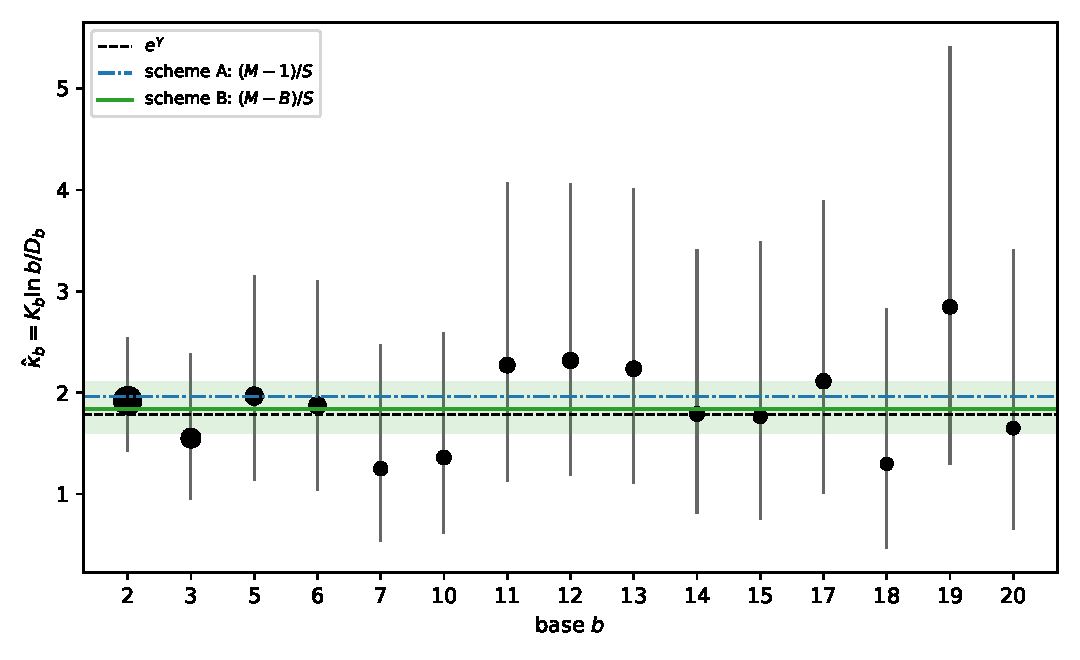
\includegraphics[width=.85\textwidth]{fig_kappa.pdf}
\caption{Per-base estimates $\hat\kappa_b$ with exact $95\%$ Garwood
intervals~\eqref{eq:garwood}; marker area is proportional to $N_b$. Dashed line: the
LPW value $\eg$; green with a band: the pooled scheme~B estimate and its interval;
blue dash-dotted: the scheme~A estimate $(M-1)/S$. Each base separately is
compatible with a universal constant.}
\label{fig:kappa}
\end{figure}

\subsection{The homogeneity test and its power}\label{sec:homog}

Let $H_0$ be the model with a single $\kappa$ and $H_1$ the model with free
$\kappa_b$. From the conditional likelihood of Proposition~\ref{prop:cond}, since
$\sum_b\hat\kappa_bD_b/\ln b=K=\hat\kappa_{\mathrm B}S$, the likelihood-ratio
statistic reduces to
\begin{equation}\label{eq:LR}
\Lambda=2\sum_b K_b \ln\frac{\hat\kappa_b}{\hat\kappa_{\mathrm B}}
=2\sum_b K_b\ln\frac{K_b}{K\,s_b/S},\qquad s_b=\frac{D_b}{\ln b}.
\end{equation}
Crucially, its null distribution is \emph{exact} here: conditioning on
$K=\sum_bK_b$ turns~\eqref{eq:pivotB} into the multinomial model
$(K_b)\mid K\sim\mathrm{Multinomial}(K;\,s_b/S)$, and there is no need to appeal
to $\chi^2_{B-1}$ asymptotics. We obtain $\Lambda=7.127$, exact $p=0.935$
($2\cdot10^6$ multinomial replications, $\pm0.0003$ at the $95\%$ level); the
asymptotic
approximation gives $p=0.930$ on $14$ degrees of freedom, that is, it works well
in this case. An exact null law exists under scheme~A as well: there, under
$H_0$, the quantities $\kappa s_b$ are independent $\Gam(N_b,1)$ variables, so the
vector $s_b/S$ is Dirichlet with parameters $N_b$ and does not depend on
$\kappa$; the analogue of statistic~\eqref{eq:LR} with $N_b$ in place of $K_b$ is
$\Lambda_{\mathrm A}=7.395$ with exact $p=0.923$ ($\chi^2$: $0.918$;
tag~[S30]).

But a non-rejection is informative exactly to the extent that the test is
powerful, and here one must apply to oneself the same requirement one applies to
the literature. We simulated alternatives in which the $\kappa_b$ are lognormally
scattered with mean $\eg$ and coefficient of variation $cv$ (that is, $\ln\kappa_b$
has variance $\ln(1+cv^2)$), conditionally on the observed $K$:
$(K_b)\mid K\sim\mathrm{Multinomial}\bigl(K;\,\kappa_bs_b/\sum_{b'}\kappa_{b'}s_{b'}\bigr)$;
the critical value is the $95\%$ quantile of the exact null law:

\begin{center}
\small
\begin{tabular}{lrrrrrrrrr}
\toprule
$cv$ & 0.05 & 0.10 & 0.15 & 0.20 & 0.25 & 0.30 & 0.35 & 0.40 & 0.50\\
power & 0.059 & 0.097 & 0.184 & 0.326 & 0.484 & 0.645 & 0.774 & 0.851 & 0.948\\
\bottomrule
\end{tabular}
\end{center}

The test attains $80\%$ power only at $cv\approx0.37$ ($12\,000$ replications
per grid point, power accurate to about $\pm0.004$). The centre of the
distribution of $\kappa_b$ (mean or median) does not affect the power: the
multinomial probabilities $\kappa_bs_b/\sum_{b'}\kappa_{b'}s_{b'}$ do not change
when all $\kappa_b$ are multiplied by the same number, and only the spread
matters. Hence $p=0.935$ means: the
data do not require base-dependent frequencies, but neither do they exclude a
spread of $\kappa_b$ with a coefficient of variation of up to a third. The
statement ``lucky bases do not exist'' does not follow from the available data;
what follows is the weaker statement ``their existence is not supported by the
data, and a spread with a coefficient of variation below $0.37$ is detected with
probability below $80\%$''.

\subsection{Robustness}\label{sec:robust}

\paragraph{Lower truncation.} We varied the lower truncation point in order to
probe the asymptotic regime (the heuristic~\eqref{eq:LPW} is asymptotic, whereas
the constant-intensity model starts at $n=2$). The results are in
Table~\ref{tab:trunc}. The scheme~A estimate grows from $1.965$ to $2.085$ in the
strictly consistent variant $N_b\ge1$ (to $2.099$ with the selection
$N_b\ge2$)---not strictly monotonically (at $n>10^{2}$ it retreats from $2.019$ to
$2.012$) but systematically: the growth is $6.1\%$ ($6.8\%$), and all values come
from nested subsamples of the same data. It is not, however, a significant trend:
simulating the data on the same origins and event counts (under scheme~B with the
frontier $W_b=N_b/\lambda_b$, the rule ``$\mathbb E[\#]$ = observed'' of
Table~\ref{tab:calib}), a rise of the scheme~A estimate by at least $6.1\%$ occurs
with probability $0.219$ under scheme~A and $0.615$ under scheme~B (with the
selection $N_b\ge2$, for a rise of $6.8\%$: $0.196$ and $0.597$; tags~[S29],
[S30]). The scheme~B estimate
shows no upward trend and stays close to $\eg$, within $1.757$--$1.871$ in the
strictly consistent variant $N_b\ge1$ (with the selection $N_b\ge2$,
$1.789$--$1.871$), and its
$p$-values lie between $0.53$ and $1.00$ at all truncation levels. The reason is
visible from~\eqref{eq:pivotB}: truncation reduces $M$ but not $B$, whereas
scheme~A subtracts one regardless of the sample size; the difference of the two
estimates is $(B-1)/S$ and grows mechanically, since $S$ falls under truncation
from about $110$ to~$42$. The truncation profile is therefore consistent with
the diagnosis of \S\ref{sec:scheme} and weakly favours scheme~B (a likelihood
ratio of about three), but it is not an independent confirmation. From $n>10$
onwards the scheme~B estimate decreases ($1.871\to1.757$, by $6.1\%$, in the
strictly consistent variant; to $1.789$ with the selection $N_b\ge2$); this too is
within the noise of nested subsamples: under scheme~B with the same frontier a fall
from $n>10$ to $n>10^4$ at least as large as the observed one occurs with
probability $0.229$, and a fall from the full sample to $n>10^4$ at least as large
as the observed one ($4.4\%$) with probability $0.306$ (with the selection
$N_b\ge2$, for a fall of $2.7\%$, $0.308$; tags~[S29], [S30]).
The second-order term does not remove this decrease (\S\ref{sec:second}). The
curves are shown in Figure~\ref{fig:trunc}.

The result does not depend on where the origin is placed either. With the origin
at the truncation point itself (the first surviving event is then not lost), the
scheme~B estimate is $1.891$, $1.867$, $1.906$ and $1.891$ at $n>10$, $10^2$,
$10^3$, $10^4$ ($p=0.43$--$0.60$). If for the five bases whose origin
$n_{\min}=2$ is fixed by arithmetic (\S\ref{sec:bases}) the origin is moved to
the second index, then $(M-B)/S=1.882$ with $p=0.457$ (tag~[S29]).

\begin{table}[t]
\centering
\caption{Robustness to lower truncation. A base is retained if at least
\emph{two} events survive the truncation ($N_b\ge2$); at $n>10^4$ base~19 no longer
meets this criterion, whence $B=14$. The criterion matters: under the weaker
requirement $N_b\ge1$ base~19 is retained, giving the last row; only that row is
strictly consistent with Proposition~\ref{prop:cond}, since selecting on
$N_b\ge2$ means selecting on $K_b\ge1$ and biases the estimate upward
(Remark~\ref{rem:selection}). The interval and $p_{\mathrm B}$ are exact,
scheme~B; the last column ($p_{\mathrm A}$, the scheme~A Gamma pivot) is given
for comparison with the old practice.}
\label{tab:trunc}
\small
\begin{tabular}{lrrrrlrr}
\toprule
truncation & $B$ & $M$ & $(M-1)/S$ & $(M-B)/S$ & 95\% CI, scheme B
& $p_{\mathrm B}$ & $p_{\mathrm A}$\\
\midrule
none & 15 & 218 & 1.9648 & 1.8381 & [1.594, 2.109] & 0.672 & 0.142\\
$n>10$ & 15 & 192 & 2.0192 & 1.8712 & [1.606, 2.168] & 0.531 & 0.080\\
$n>10^2$ & 15 & 156 & 2.0116 & 1.8299 & [1.540, 2.158] & 0.771 & 0.124\\
$n>10^3$ & 15 & 125 & 2.0551 & 1.8231 & [1.498, 2.197] & 0.832 & 0.106\\
$n>10^4$ & 14 & 89 & 2.0990 & 1.7889 & [1.407, 2.242] & 1.000 & 0.116\\
\midrule
$n>10^4$, $N_b\ge1$ & 15 & 90 & 2.0848 & 1.7569 & [1.382, 2.202] & 0.966 & 0.128\\
\bottomrule
\end{tabular}
\end{table}

\begin{figure}[t]
\centering
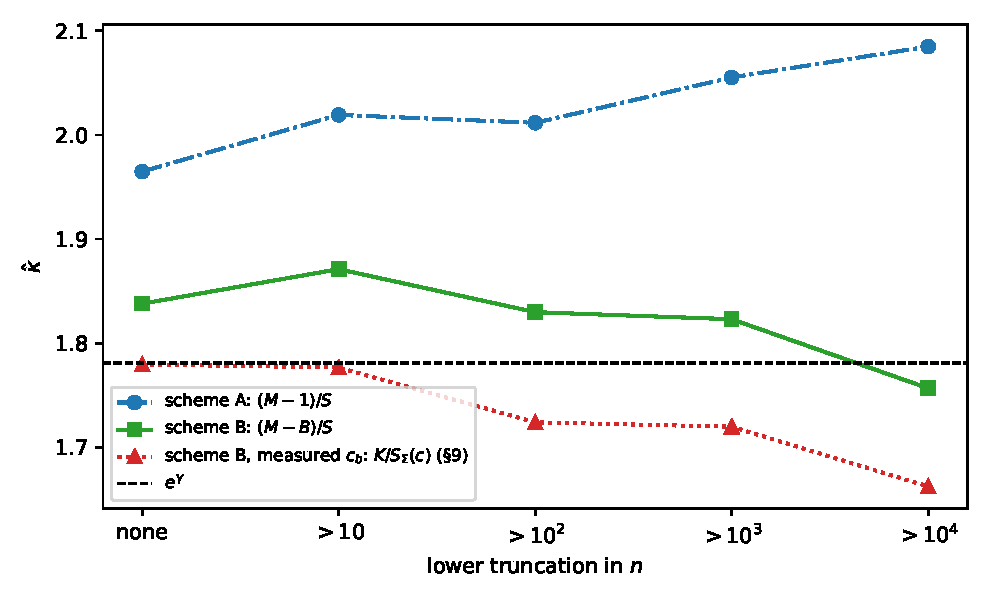
\includegraphics[width=.75\textwidth]{fig_truncation.pdf}
\caption{The pooled estimate under lower truncation: $(M-1)/S$ (scheme~A),
$(M-B)/S$ (scheme~B) and $K/S_\Sigma(c)$ with the measured second-order term and
the exposure summed over the primes (\S\ref{sec:second}). The last point
($n>10^4$) is the strictly consistent variant $N_b\ge1$ (Table~\ref{tab:trunc}).
The upward trend of scheme~A disappears under scheme~B. All curves come from nested subsamples, and
their changes under truncation are within the noise (\S\ref{sec:robust}).}
\label{fig:trunc}
\end{figure}

\paragraph{Leave-one-base-out.} A leave-one-base-out analysis gives
$\hat\kappa_{\mathrm B}$ within $[1.808,\,1.878]$ (the extreme values arise when
$b=19$ and $b=3$ are removed) and exact $p$-values within
$[0.49,\,0.85]$; no single base determines the conclusion.

\paragraph{Status of the data.} Restricting base~2 to the fifty double-checked
exponents moves the scheme~B estimate from $1.838$ to $1.834$ (scheme~A: from
$\tilde\kappa=1.965$, $p=0.142$ to $\tilde\kappa=1.961$, $p=0.151$). PRP status
begins far below one million for most terms (\S\ref{sec:data}), so the next
variant tests not PRP status as such but the most recent and least re-checked
finds: excluding all indices $n>10^6$ gives $M=182$ and $(M-B)/S=1.800$
($\tilde\kappa=1.951$). In the worst case, when the last known PRP of some base
turns out to be composite, the largest shift comes from $b=17$: $(M-B)/S=1.848$
($\tilde\kappa=1.977$). All variants lie inside both interval~\eqref{eq:resA} and
interval~\eqref{eq:resB}, so possible pseudoprimes do not affect the conclusion.
More important than spurious finds are missed ones (\S\ref{sec:data}): a miss
lowers $K$ at unchanged $S$ and biases the estimate downward, in the direction of
the main conclusion. For LPW to be rejected from above, at least $23$ finds would
have to be missing inside the windows, $1.5$ per base, and at least $30$ with the
second-order term (tag~[S30]). The two 2024 finds for base~5 do not fall inside
the windows: they lie above $n_{\max}$, beyond an unsearched gap
(\S\ref{sec:data}).

\section{Statistical power}\label{sec:power}

By~\eqref{eq:pivotB} the power against a true constant $\kappa=r\eg$ at level
$\alpha$ is available in closed form (Table~\ref{tab:power}). The convention has
to be stated: throughout this work the test is \emph{two-sided}, with the
doubled-minimum-tail convention, $\alpha=0.05$. The one-sided variant of the same
test gives noticeably different numbers; they are shown in the right-hand part
of the table for comparability with works in which the convention is not stated.

\begin{table}[t]
\centering
\caption{Power at level $\alpha=0.05$ for rejecting $\kappa=\eg$ when the true
constant exceeds it by the stated factor. Exposures: $S_2=26.02$ ($K=50$) for base~2
alone and $S=110.44$ ($K=203$) for the pooled sample.}
\label{tab:power}
\small
\begin{tabular}{lrr@{\qquad}rr}
\toprule
& \multicolumn{2}{c}{two-sided} & \multicolumn{2}{c}{one-sided}\\
\cmidrule(r){2-3}\cmidrule(l){4-5}
$\kappa/\eg$ & Mersenne only & pooled & Mersenne only & pooled\\
\midrule
1.05 & 0.060 & 0.099 & 0.082 & 0.165\\
1.10 & 0.099 & 0.266 & 0.147 & 0.386\\
1.15 & 0.164 & 0.514 & 0.235 & 0.644\\
1.20 & 0.253 & 0.752 & 0.343 & 0.844\\
1.30 & 0.479 & 0.972 & 0.581 & 0.988\\
1.50 & 0.861 & 1.000 & 0.910 & 1.000\\
\bottomrule
\end{tabular}
\end{table}

At $80\%$ power the Mersenne sequence alone detects only deviations of $45.5\%$
and above; pooling fifteen bases lowers that threshold to $21.3\%$ (one-sided
variant: to $18.7\%$). Table~\ref{tab:power} concerns an excess; for a deficit
of the constant the thresholds of the same two-sided test differ: $37.4\%$ for
base~2 alone and $19.2\%$ for the pooled sample (tag~[S29]). Attaining $80\%$ power against a $10\%$ deviation requires
an exposure $S\approx470$, that is, $K\approx837$ conditional events
($M\approx852$) at $\kappa=\eg$ (if the true constant is $10\%$ larger, one
expects $K\approx921$ conditional events, that is, $M\approx936$ finds); against $5\%$, $S\approx1823$ and $K\approx3246$.
The power function of a discrete test is not monotone in $S$ (it is
saw-toothed), so the values given are those beyond which the power no longer
drops below $80\%$ (found by an exhaustive scan over $S$ with step $0.01$).

These thresholds are computationally out of reach, and it is worth saying by how
much. Since $K$ grows logarithmically in the search frontier, doubling the
frontiers \emph{of all fifteen bases} adds $\ln2\sum_b1/\ln b=5.41$ to the
exposure, that is, on average $\eg\cdot5.41=9.64$ conditional events. To raise
the exposure from $110.4$ to $470$ one needs $(470-110.4)/5.41\approx66.4$
doublings, that is, a growth of the frontiers by a factor of about
$2^{66.4}\approx10^{20}$; for a sensitivity of $5\%$, about $316$ doublings, that
is, a factor of order $10^{95}$. This is not a
matter of decades but of magnitudes lying beyond the reach of any conceivable
computation. Both power curves, as functions of the true deviation, are shown in
Figure~\ref{fig:power}.

\begin{figure}[t]
\centering
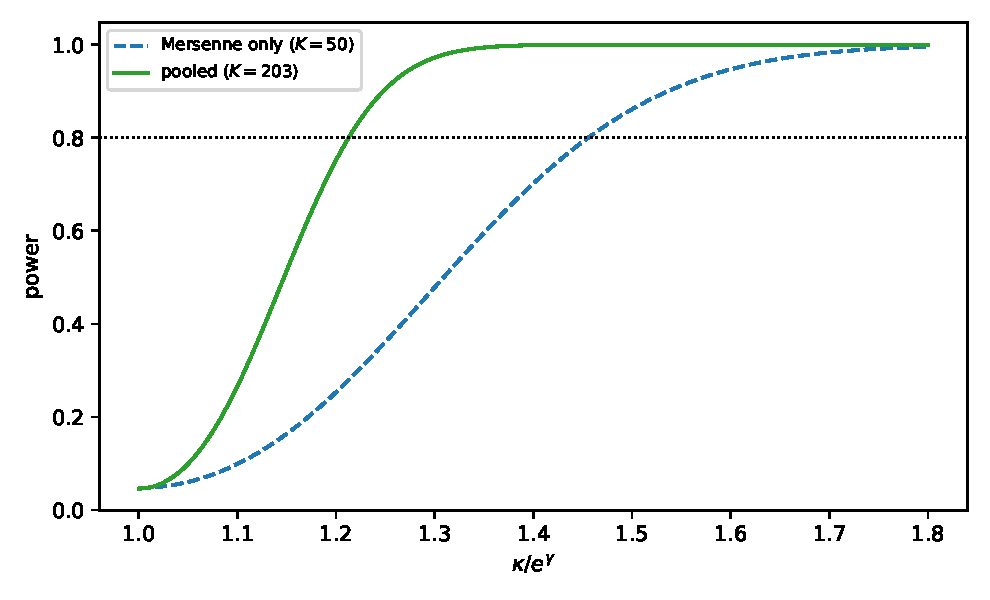
\includegraphics[width=.72\textwidth]{fig_power.pdf}
\caption{Power of the two-sided rejection of $\kappa=\eg$ at level $\alpha=0.05$.
The horizontal line marks $80\%$ power.}
\label{fig:power}
\end{figure}

This yields a rule for reading this literature. A report that the data agree with LPW
to within a few percent is not evidence for LPW at the level of a few percent;
it is compatible with a constant that is wrong by a factor of one and a half.
The pooled analysis does, however, establish a genuine bound: the universal
constant, if it exists, lies under (A1) roughly in $[1.59,\,2.11]$ in the
constant-intensity model and in $[1.52,\,2.06]$ with the measured second-order
term at $n>10$ (\S\ref{sec:second}); no base deviates from it detectably.

\section{The same error in a different guise}\label{sec:sameerror}

The Mersenne counting function invites a related error, which we present as a
worked example. Regressing $\pi_2(t)$ on $t$ at the event points, over the $50$
double-checked exponents (numbered $0,\dots,N-1$: the smallest exponent is the
origin, not an event), gives a slope of $2.6391$ and an intercept of $-2.9627$
with an OLS standard error of $0.4469$---apparently significant, and suggestive
of a secondary term in~\eqref{eq:LPW}. Nothing of the sort.

Two defects compound. The residuals of the cumulative count are strongly
autocorrelated, here $\rho_1=0.825$ (the sample correlation of adjacent
residuals; the sample autocorrelation function gives $0.751$); the Newey--West
estimator with the Bartlett kernel and eight lags, without a degrees-of-freedom
correction, raises the standard error to $0.7315$ (with the correction $n/(n-k)$,
to $0.7466$; tag~[S30]). More importantly, the
regression uses only the event points and thereby discards the empty interval
between the last exponent and the search frontier. The correct null model holds
the interval $[t_0,T]$ fixed, where $T=\ln X_{\mathrm{ver}}$, and conditions on
exactly $N-1=49$ events strictly to the right of $t_0$, which, by the
order-statistics property of the Poisson process given the number of events
(cf.\ the proof of Proposition~\ref{prop:unbiased}(b)), means $49$ independent
uniform points on $(t_0,T]$. Over $60\,000$ such replications the intercept has
median $-1.529$ and a $5$--$95\%$ range of $[-5.99,\,2.20]$, giving a two-sided
$p=0.570$ for the observed value. The secondary term is an artifact of
conditioning. Note that even the correct null distribution is not centred at
zero. The count vanishes at $t_0=\ln2$, while the intercept is measured at
$t=0$, and this alone shifts it by about $-\hat\lambda\ln2$, that is, by almost
$-1.9$. Comparing $-2.96$ with zero is thus doubly wrong: because of the
understated standard error, and because the null expectation is not zero.

\subsection{Three consequences of one and the same conditioning}

\paragraph{(i) The bootstrap does not help.} The natural reaction to a
suspiciously small OLS standard error is a nonparametric pairs bootstrap over the
event points. On
the base-2 data, a bootstrap over $20\,000$ resamples gives median $-2.948$,
standard deviation $0.385$ and a $95\%$ interval $[-3.809,\,-2.300]$ lying
entirely below zero; the proportion of negative values is $100\%$. This is not a
confirmation but a repetition of the same error: resampling the observed points
reproduces the variability within the realized configuration and cannot recover
the variability of the process that produced that configuration. The correct
null distribution has standard deviation $2.499$ ($5.6$ times the OLS standard
error of $0.447$), that is, it is $6.5$ times
wider than the bootstrap one \emph{in terms of standard deviation} (and likewise
$6.5$ times in terms of the width of the $95\%$ interval).

\paragraph{(ii) Spurious underdispersion.} Comparing the observed
$\max_i|r_i|=6.347$, where $r_i=i-\hat\lambda(t_i-t_0)$, with a simulation of an
\emph{unconditioned} Poisson process suggests the conclusion that the counting
function is ``smoother than Poisson''. Against the correct null
distribution---conditioning on $N-1$ events and estimating $\lambda$ from the
last of them---the median is $5.117$ and the two-sided significance level is
$0.529$. The observation is entirely ordinary. An unnormalized supremum is
insensitive near the pinned ends, so we also checked the version standardized by
the bridge variance, $\max_i|r_i|/\sqrt{(N-1)u_i(1-u_i)}$ with
$u_i=(t_i-t_0)/(t_{N-1}-t_0)$ over the interior events, under the same null law:
it gives $3.45$ with $p=0.194$, again an ordinary value (tag~[S29]).

\paragraph{(iii) The ``mid-range deficit''.} Estimating $\lambda$ from the last
event forces the residual $r$ to vanish at both ends ($r(t_0)=r(t_N)=0$ under
the correct numbering), turning its trajectory into an analogue of a Brownian
bridge. Pinning the ends sets the typical size of an excursion in the middle of
the range, but not its sign: the bridge is asymptotically symmetric (with
$N-1=49$ the asymmetry is negligible), and a negative excursion is no more likely
than a positive one of the same size. The observed mean of the residuals $r_i$ at
the events in the middle half of the $t$-axis, that is, with
$u_i\in[1/4,3/4]$, is
$-3.13$ against a simulation median of $-0.012$ and $p=0.272$; the proportion of
replications with a negative mean excursion is $0.502$, so there is no
systematic deficit. The trajectory of the residual process itself, together with
the simulation band, is shown in Figure~\ref{fig:bridge}.

\begin{figure}[t]
\centering
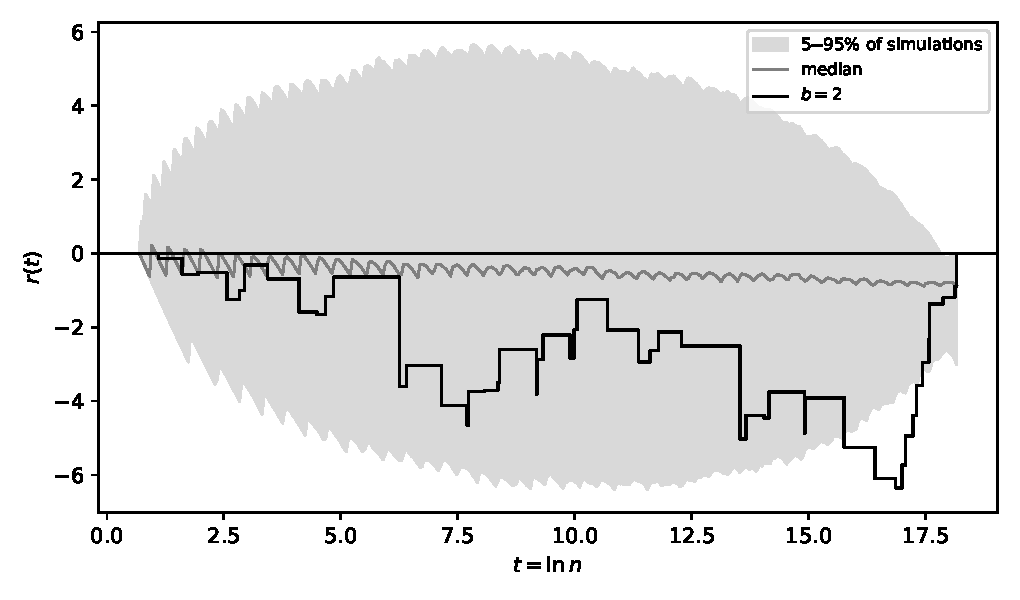
\includegraphics[width=.78\textwidth]{fig_resid_bridge.pdf}
\caption{The residual process $r(t)$ for base $b=2$ together with the pointwise
$5$--$95\%$ quantile band and the median of the simulations. The band is built for
the same step function $r(t)=\#\{t_i\le t\}-\hat\lambda(t-t_0)$ under the null law of
\S\ref{sec:sameerror}: $49$ uniform points on $(t_0,\ln X_{\mathrm{ver}}]$,
$\hat\lambda$ from the last of them. The trajectory leaves the band near
$t\approx16.9$, where $r=-6.35$ against a pointwise $5\%$ quantile of $-3.85$ (the
band drawn; an independent simulation~[S29] gives $-3.81$). A
pointwise exit says nothing about significance: for the whole trajectory the
standardized supremum gives $p=0.194$, the plain one $p=0.529$
(\S\ref{sec:sameerror}, tag~[S29]).}
\label{fig:bridge}
\end{figure}

\subsection{Base 2 at a known frontier}

Base~2 is one of the two bases of the main set with a published frontier (the
other is $b=10$, \S\ref{sec:frontiers}); for it a scheme~B analysis is possible
\emph{using the full exposure} rather than only the conditional one. With
$T=\ln X_{\mathrm{ver}}$ we obtain
$\hat\lambda=(N-1)/(T-t_0)=2.7960$ against $\eg/\ln2=2.5695$, that is,
$\hat\kappa_2=1.9381$ with an exact $95\%$ Garwood interval $[1.434,\,2.562]$
and a Poisson $p$-value of $0.593$ (doubled tail; under the mid-$p$ convention,
$0.545$---the convention must be stated here, since the difference is
appreciable). The conditional estimate on \emph{the same slice of data}---the
same $50$ double-checked exponents---gives $1.9046$; the difference is small
because the last exponent of that slice, $77\,232\,917$, happens to lie very
close to the frontier $81\,648\,221$. (For comparison, the conditional estimate
over all $52$ known exponents, reported in Table~\ref{tab:bases}, is $1.9215$;
it must not be compared with $\hat\kappa_2$, being a different sample.) This is
a coincidence of one realization, not a property of the method: the correction
of~\S\ref{sec:cost} concerns the average over the position of the last event
relative to the frontier.

We note in passing that the regime described here is exactly the one to which
we urge a transition for all bases: with $W_b$ known, conditioning on $D_b$
becomes unnecessary, and the precision increases by the very $3.7\%$ discussed
in~\S\ref{sec:exact}.

\subsection{The sign of the intercept proves nothing}

The previous version gave here an ``independent argument'': that the theoretical
secondary term, $(\eg/\ln2)\mathfrak M=+0.672$ with the Meissel--Mertens constant
$\mathfrak M=0.26150\ldots$, has the sign opposite to the observed $-2.963$. This
argument is wrong, and we withdraw it: it takes into account only one of the two
Mertens theorems. Summing~\eqref{eq:probp} over primes $p\le x$ with
$\sum_{p\le x}\ln p/p=\ln x+E+o(1)$, $E=-1.3326\ldots$, and
$\sum_{p\le x}1/p=\ln\ln x+\mathfrak M+o(1)$ gives
\[
\pi_2(x)\approx\frac{\eg}{\ln2}\bigl(\ln x+c_2\ln\ln x\bigr)+C_0,\qquad
C_0=\frac{\eg}{\ln2}\bigl(E+c_2\mathfrak M\bigr).
\]
With the measured $c_2=0.96$ (\S\ref{sec:second}) we get $C_0=-2.78$; direct
summation over $p\le10^8$ gives the same value. The constant $C_0$ itself depends
strongly on the treatment of small $p$, where probability~\eqref{eq:probp}
exceeds one: with the probabilities capped at one it becomes $C_0=-5.05$
(tag~[S30]). The intercept of the regression is even less $C_0$: it depends in
addition on the numbering of events, on the linearization of the term
$c_2\ln\ln x$ and on the conditioning on the number of events. A direct check is
more reliable. Let the heuristic itself generate the Mersenne
exponents---Bernoulli trials over the primes $p\le X_{\mathrm{ver}}$ with
probability~\eqref{eq:probp} at the measured $c_2$---and condition on $50$
events. The intercept of the same regression then has median $-2.52$ and a
$5$--$95\%$ range of $[-5.20,\,-0.15]$, and the observed $-2.963$ lies at its
quantile $0.385$; with Wagstaff's refinement ($a=2$ or $6$) the median is
$-2.32$ and the quantile $0.343$ (tag~[S28]). The second-order heuristic predicts
a negative intercept of the same size as the observed one. What bears on the
structure is not the sign of $C_1$ but only the correct null distribution
(\S\ref{sec:sameerror}, $p=0.57$): the intercept $C_1$ is a parameter of the fit
and calls for no substantive interpretation.

\section{Structural corrections}\label{sec:struct}

Consider the more general parametrization of the intensity
$\lambda_b=(\kappa/\ln b)\,C_b$ and four models for the factor:
\begin{align*}
\text{I:}&\quad C_b=1;\\
\text{II:}&\quad C_b=\prod_{p\mid b-1,\ p\ne2}\Bigl(\tfrac{p}{p-1}\Bigr)^{\alpha}
                 \prod_{p\mid b+1,\ p\ne2}\Bigl(\tfrac{p}{p-2}\Bigr)^{\beta};\\
\text{III:}&\quad C_b=\prod_{p\mid b^2-1}\Bigl(\tfrac{p}{p-1}\Bigr)^{\eta};\\
\text{IV:}&\quad C_b=\exp\bigl(\theta_1\omega(b-1)+\theta_2\omega(b+1)+\theta_3\ln b\bigr).
\end{align*}
The models are numbered with Roman numerals so as not to confuse them with the
observation schemes~A and~B; the exponent in model~III is written $\eta$ so as
not to confuse it with the Euler constant or with the distance to the frontier
$\delta_b$. The likelihood here is the \emph{conditional
Poisson} likelihood of Proposition~\ref{prop:cond},
$\ell_{\mathrm B}=\sum_b\bigl[K_b\ln\mu_b-\mu_b-\ln K_b!\bigr]$ with
$\mu_b=\kappa C_b D_b/\ln b$; the previous version used the scheme~A
likelihood~\eqref{eq:loglik}, which is incompatible with \S\ref{sec:scheme}. The
results are in Table~\ref{tab:struct}. No parametrization gives a significant
improvement; the BIC-based Bayes factors at $n=K=203$ strongly support the base
model against models~II and~IV ($112$ and $1112$) and moderately against~III
($10.6$; at $n=15$, $2.9$; tag~[S30]).

Models~II--IV formalize the folklore notion of ``lucky'' bases through the
divisors of $b\pm1$, after the pattern of a Hardy--Littlewood singular series.
Theory predicts no such factor: for an odd prime $p\nmid b-1$ the primes
$q\mid b-1$ and $q\mid b+1$ do not divide $\Rb(p)$, since $\Rb(p)\equiv p$ and $\Rb(p)\equiv1\pmod q$ respectively, but all
primes $q<2p+1$ behave in the same way for every~$b$ (\S\ref{sec:data}), and this
gain is already part of the common factor $\eg\ln(2p)$. The heuristic predicts
$C_b\equiv1$, so this section tests the folklore rather than the theory; the
substantive second-order dependence on the base is analysed
in~\S\ref{sec:second}.

\begin{table}[t]
\centering
\caption{Comparison of structural models under the conditional Poisson likelihood of
Proposition~\ref{prop:cond} (full form, including $-\ln K_b!$); LR and $p$ are
relative to model~I; BIC is computed with $n=K=203$.}
\label{tab:struct}
\small
\begin{tabular}{lrrrrrrr}
\toprule
Model & parameters & $\ln L$ & LR & $p$ & AIC & BIC & $P(\text{model}\mid\text{data})$\\
\midrule
I & 1 & $-35.753$ & --- & --- & 73.51 & 76.82 & 0.906\\
II & 3 & $-35.162$ & 1.18 & 0.554 & 76.32 & 86.26 & 0.008\\
III & 2 & $-35.458$ & 0.59 & 0.443 & 74.92 & 81.54 & 0.085\\
IV & 4 & $-34.797$ & 1.91 & 0.591 & 77.59 & 90.85 & 0.001\\
\bottomrule
\end{tabular}
\end{table}

\begin{remark}[Sensitivity of the BIC]
The choice of effective sample size for the BIC is not obvious: the likelihood
has $B=15$ independent summands, but the information grows as $K=203$. With
$n=15$ the posterior probabilities are $0.661$ / $0.080$ / $0.229$ / $0.030$;
with $n=203$ they are $0.906$ / $0.008$ / $0.085$ / $0.001$. The conclusion
favors model~I under either choice, but with $n=203$ it is substantially
stronger. We report $n=K$ as matching the number of independent conditional
events.
\end{remark}

\paragraph{A fixed arithmetic correction.} We considered separately a model with
a \emph{fixed} (not estimated) factor
$C^{\mathrm{fix}}_b=\prod_{p\mid b-1,p\ne2}\frac{p}{p-1}\prod_{p\mid b+1,p\ne2}\frac{p}{p-2}$,
whose mean over the fifteen bases is $2.462$. It gives $\hat\kappa=0.759$. We
stress that comparing this value with $\eg$ is meaningless: in the
reparametrized model $\kappa$ has a different scale, and such a ``goodness-of-fit
test'' would only be testing whether the mean of $C_b$ equals one. Since models
I and $C^{\mathrm{fix}}$ are non-nested and have the same number of free
parameters, the correct comparison is directly by likelihood: $\ln L=-51.53$
against $-35.75$, a difference of $-15.78$. The fixed correction is decisively
rejected.

\paragraph{Logarithmic corrections.} A substantive correction is needed here.
The model $\lambda_b(t)=(\kappa/\ln b)(1+c_1/t+c_2/t^2)$ used in the previous
version is \emph{not an admissible intensity}: at the estimates obtained there,
$\hat c_1=+0.108$, $\hat c_2=-0.826$, the factor vanishes at $t=0.8564$ and is
negative to the left of that point, that is, for $n<2.355$; in particular, at
$t_0=\ln 2$ it equals $-0.5634$. The bases with $n_{\min}=2$
($b=2,6,10,12,18$) integrate the intensity over a region where it is negative,
and the measure $\int\lambda\,dt$ is negative on that stretch. That the
likelihood could be computed at all was a matter of chance: the smallest index
that is an event is $3$, that is, $t=1.0986>0.8564$, so no negative values fell
under the logarithm.

The correct parametrization of the same family is
\begin{equation}\label{eq:logcorr}
\lambda_b(t)=\frac{\kappa}{\ln b}\exp\Bigl(\frac{c_1}{t}+\frac{c_2}{t^2}\Bigr),
\end{equation}
which is identically positive and reduces to the null model at $c_1=c_2=0$. It
is estimated by the conditional point-process likelihood~\eqref{eq:condinhom}:
the sum $\sum\ln\lambda(t_i)$ is taken over the events \emph{excluding the last},
and the integral $\int\lambda$ runs from $t_0$ to the last event $t_0+D_b$, not
to the unknown frontier (Remark~\ref{rem:inhom}; the likelihood of the count
alone is inadmissible here: it discards the positions of the events, which are
the only thing that determines $c_1,c_2$). The result: $\hat\kappa=1.748$,
$\hat c_1=0.75$, $\hat c_2=-1.44$; the likelihood ratio against $c_1=c_2=0$ is
$2.03$ on two degrees of freedom, $p=0.36$ (tag~[S17]). Since $\hat c_1$ and
$\hat c_2$ are strongly correlated, the $\chi^2_2$ asymptotics are not guaranteed
here, and we calibrated them by a parametric bootstrap of the conditional model:
$p=0.366$ from $10\,000$ replications, $95\%$ quantile $5.93$ against $5.99$ for
$\chi^2_2$ (tag~[S30]). There is no significant improvement. The estimate $\hat c_1$ is strongly correlated with $\hat c_2$ here
and is not informative on its own: the one-parameter model~\eqref{eq:lam2} on the
same data gives $\hat c=-0.40$ in the integral form and $1.03$ with the exposure
summed over the primes (\S\ref{sec:second}).

\section{The second-order term of the heuristic itself}\label{sec:second}

So far we have tested the constant-intensity model~\eqref{eq:lam}. But the LPW
heuristic itself predicts an intensity that is \emph{not} constant at
finite~$n$, and this changes the meaning of comparing $\hat\kappa$ with $\eg$.

\paragraph{Derivation.} Let $p$ be an odd prime, $p\nmid b-1$, and let $q$ be a prime
divisor of $\Rb(p)$. Then $b$ has order $p$ modulo $q$, whence $q\equiv1\pmod p$,
and since $\Rb(p)$ is odd, $q\equiv1\pmod{2p}$. Hence $\Rb(p)$ has no prime
divisors below $2p+1$, and by Mertens' theorem the probability of primality is
increased by the factor $\prod_{q<2p}(1-1/q)^{-1}\approx\eg\ln(2p)$ compared with
a random number of the same size. This is the derivation
of~\cite{wagstaff1983,t5k}:
\begin{equation}\label{eq:probp}
\Pr\bigl(\Rb(p)\ \text{prime}\bigr)\approx\frac{\eg\ln(a_bp)}{p\ln b}.
\end{equation}
Wagstaff's refinement for $b=2$ takes into account that $q\equiv\pm1\pmod8$ and
gives $a=2$ for $p\equiv3\pmod4$ and $a=6$ for $p\equiv1\pmod4$. In the
continuous approximation, multiplying~\eqref{eq:probp} by the density of primes
$1/\ln n$ and passing to
$t=\ln n$, we get
\begin{equation}\label{eq:lam2}
\lambda_b(t)=\frac{\kappa}{\ln b}\Bigl(1+\frac{c_b}{t}\Bigr),\qquad
c_b=\langle\ln a_b\rangle,\qquad \kappa=\eg,
\end{equation}
and, for the counting function,
$\pi_b(x)\approx(\eg/\ln b)\,(\ln x+c_b\ln\ln x)$. The
asymptotics~\eqref{eq:LPW} are unaffected, but at $t\approx10$--$18$ the
correction $c_b/t$ amounts to several percent---as much as the effects
discussed in this paper.

\paragraph{Calibration of $c_b$.} Wagstaff's device---replacing $a_b$ by the
smallest admissible divisor candidate---is crude, and we estimate $c_b$ from the
actual divisibility of $\Rb(p)$ within the same Mertens heuristic. For a random
number $N$, by Mertens,
\[
\Pr(N\ \text{prime}\mid\text{no prime divisors}<Y)\approx\eg\ln Y/\ln N.
\]
Hence $\Pr(\Rb(p)\ \text{prime})\approx F_b(p,Y)\,\eg\ln Y/(p\ln b)$, where
$F_b(p,Y)$ is the indicator that $\Rb(p)$ has no prime divisors below $Y$.
Comparison with~\eqref{eq:probp} gives
\begin{equation}\label{eq:cbemp}
c_b(Y)=\bigl\langle F_b(p,Y)\ln Y-\ln p\bigr\rangle_p .
\end{equation}
The indicator $F_b$ is computed \emph{exactly}. For $p>b$, $\Rb(p)$ has a prime
divisor below $Y$ if and only if $b^p\equiv1\pmod q$ for some $q=2kp+1<Y$, prime
or not. Indeed, the prime divisors of such a $q$ that do not divide $b-1$ are
congruent to $1$ modulo $p$ and divide $\Rb(p)$; the part of $q$ composed of
divisors of $b-1$ divides $b-1<p$ by the lifting-the-exponent lemma and is
congruent to $1\pmod p$, hence equals~$1$. For $31\,598$ primes
$p\in[2\cdot10^4,\,4\cdot10^5)$ and $Y=100p$, $1000p$, $3000p$ we obtain values
of $c_b$ that are stable in $Y$ to within a standard error of $0.05$ (script
\texttt{cb\_empirical.py}, tag~[S19]; the values for different $Y$ are obtained
on the same set of $p$ and are therefore correlated). At $Y=1000p$ they range
from $0.43$ ($b=12$) to $1.11$ ($b=20$), with mean $0.67$. For ten bases out of
fifteen the estimate of $c_b$ is \emph{below} $\ln2\approx0.693$---the value
given by a naive application of Mertens' theorem to the single condition
$q\equiv1\pmod{2p}$; consequently, $\ln2$ is not a lower bound for the effective
$c_b$. Wagstaff's device (averaging $\ln a_b$ taking into account that $b$ is a
quadratic residue modulo~$q$) gives systematically larger values, from $1.23$ to
$1.74$ (tag~[S14]); even for $b=2$ it gives $1.242=\tfrac12(\ln2+\ln6)$ against
$0.96\pm0.05$. Moreover, this device is ambiguous: candidates divisible by a
prime divisor of $b$ are discarded, whereas those divisible by other small
primes are not; thus for $b=18$ the residue condition coincides with the one for
$b=2$, yet $c_{18}=1.646$ against $c_2=1.242$. Below, the calibration of
$c_b$ by~\eqref{eq:cbemp} is taken as the main one, and Wagstaff's variant is
given only for comparison.

\paragraph{Where the values of $c_b$ come from.} The calibration can be predicted
without computing $b^p\bmod q$ (script \texttt{cb\_theory.py}, tag~[S23]). A
prime $q=2kp+1$ divides $\Rb(p)$ if and only if $b$ lies in the subgroup of
index $2k$ of $\mathbb F_q^{*}$. A necessary condition is that $b$ be a
quadratic residue modulo~$q$, and this is determined by the Jacobi symbol
$(b/q)$. Within the subgroup of residues the natural heuristic is uniformity,
which gives the probability $2/(2k)=1/k$; for $k=1$ this equals $1$, which is
the classical case $2p+1\mid M_p$ for $p\equiv3\pmod4$. Hence the prediction
\begin{equation}\label{eq:cbth}
F^{\mathrm{th}}_b(p,Y)=\prod_{\substack{k<Y/(2p):\ q=2kp+1\ \text{prime},\\ (b/q)=+1}}
\Bigl(1-\frac1k\Bigr),\qquad
c^{\mathrm{th}}_b=\bigl\langle F^{\mathrm{th}}_b(p,Y)\ln Y-\ln p\bigr\rangle_p ,
\end{equation}
which uses only the primality of the numbers $2kp+1$ and the quadratic
character of~$b$. Table~\ref{tab:cbth} compares it with the calibration on the
same $31\,598$ primes $p$. The correlation is $0.976$ and the mean difference is
$+0.017$. A paired test over the individual~$p$ gives $\sum z_b^2=23.5$ with $15$
degrees of freedom, $p=0.074$. The prediction explains $95\%$ of the
between-base variation of $c_b$. The largest deviation is at $b=2$ ($+0.12$,
$z=2.6$); its natural source is the biquadratic character of $2$ (Gauss's
criterion), which the model does not take into account. Equation~\eqref{eq:cbth}
also implies a structural conclusion: in this approximation $c_b$ depends only
on the squarefree part of $b$. The pairs $2$ and $18$, $3$ and $12$, $5$ and $20$
have identical predictions, and the calibration confirms this within the
errors. Thus the values of $c_b$---and the fact that Wagstaff's device
overstates them---are explained by the distribution of primes of the form
$2kp+1$ and by quadratic reciprocity, not by peculiarities of the data.

\begin{table}[t]
\centering
\caption{The second-order term $c_b$: calibration from the actual divisibility
(equation~\eqref{eq:cbemp}, tag~[S19]) and the prediction~\eqref{eq:cbth} from the primality
of $2kp+1$ and the symbol $(b/q)$ (tag~[S23]); $z$ is the paired $z$-statistic of
the difference; $31\,598$ primes $p\in[2\cdot10^4,\,4\cdot10^5)$, $Y=1000p$.}
\label{tab:cbth}
\small
\setlength{\tabcolsep}{2.6pt}
\begin{tabular}{lrrrrrrrrrrrrrrr}
\toprule
$b$ & 2 & 3 & 5 & 6 & 7 & 10 & 11 & 12 & 13 & 14 & 15 & 17 & 18 & 19 & 20\\
\midrule
calibration & 0.96 & 0.44 & 1.06 & 0.59 & 0.49 & 0.55 & 0.47 & 0.43 & 0.67 & 0.53 & 0.54 & 0.76 & 0.86 & 0.54 & 1.11\\
prediction & 0.84 & 0.46 & 1.01 & 0.50 & 0.51 & 0.52 & 0.53 & 0.46 & 0.75 & 0.51 & 0.52 & 0.71 & 0.84 & 0.54 & 1.01\\
$z$ & $+2.6$ & $-0.4$ & $+1.1$ & $+2.0$ & $-0.5$ & $+0.7$ & $-1.3$ & $-0.8$ & $-1.8$ & $+0.4$ & $+0.3$ & $+1.0$ & $+0.4$ & $-0.1$ & $+2.0$\\
\bottomrule
\end{tabular}
\end{table}

\paragraph{Conditional inference for a given $c$.} By
Remark~\ref{rem:inhom}, conditionally on $D_b$ the interior events form a
Poisson process with the same intensity on $(t_0,t_0+D_b)$. But the
heuristic~\eqref{eq:probp} assigns a probability not on the $t$-axis but to each
prime index, and the expected number of events in the window is a \emph{sum over
the primes}. Proposition~\ref{prop:cond} therefore carries over in the form
\begin{equation}\label{eq:pivotc}
K\mid(D_b)_b\sim\Pois\bigl(\kappa S_\Sigma(c)\bigr),\qquad
S_\Sigma(c)=\sum_b\frac{1}{\ln b}\sum_{\substack{n_{\min}<p<n_{\max}\\ p\ \text{prime}}}
\frac{\ln p+c_b}{p},
\end{equation}
where the inner sum omits the deterministically composite cases $p\mid b-1$ and
$p=s$ (Aurifeuillean, \S\ref{sec:bases}). The estimator is $K/S_\Sigma(c)$, and
the Garwood interval~\eqref{eq:garwood} applies with $S$ replaced by
$S_\Sigma(c)$. The Poisson law~\eqref{eq:pivotc} is exact for a Poisson process
with intensity~\eqref{eq:lam2}. If the heuristic is read literally, as Bernoulli
trials at the prime indices with probabilities~\eqref{eq:probp} capped at one,
conditioning on the last find remains valid (the trials before it are independent
of that event), but the conditional law of $K$ becomes Poisson-binomial:
$\operatorname{Var}(K\mid D)/\mathbb E[K\mid D]=0.934$ on the full sample and
$0.973$ at $n>10$ (tag~[S30]). The Poisson intervals and $p$-values are therefore
conservative: the standard deviation is overstated by $3.5\%$ and $1.4\%$. A
crude allowance for the primality of the numbers $2p+1$, which is common to all
bases, brings the variance-to-mean ratio back close to one (Remark~\ref{rem:indep}). The continuous approximation~\eqref{eq:lam2} replaces this sum by
an integral:
\begin{equation}\label{eq:pivotcint}
S(c)=\sum_b\frac{D_b+c_b\ln\bigl((t_0+D_b)/t_0\bigr)}{\ln b}.
\end{equation}
It is exact only asymptotically. By Mertens' first theorem
$\sum_{p\le x}\ln p/p=\ln x+E+o(1)$ with $E=-1.3326\ldots$, and for origins
$n_{\min}=2$--$19$ the integral overstates the exposure of a base by
$0.39$--$1.42$ in $t$, $1.04$ on average; under lower truncation $n>10^2$ the
difference is below one percent (tag~[S26]). The previous version used
form~\eqref{eq:pivotcint}, which on the full sample and at $n>10$ understated the
estimate by $9.0\%$ and $3.8\%$ respectively; below, form~\eqref{eq:pivotc} is
taken as the main one.

\begin{table}[t]
\centering
\caption{Conditional inference with the second-order term: the estimate
$\hat\kappa$ and the exact two-sided $p$ against $\kappa=\eg$. ``$c{=}0$'' is the
constant-rate model; ``meas., $\int$'' are the measured $c_b$ (tag~[S19]) with the
integral exposure~\eqref{eq:pivotcint} of the previous version; ``meas., $\Sigma$''
are the same $c_b$ with the exposure~\eqref{eq:pivotc} summed over the primes (the
main variant); ``W, $\Sigma$'' is Wagstaff's device with the same sum. Truncation
as in Table~\ref{tab:trunc}. Tags~[S20], [S26].}
\label{tab:second}
\small
\setlength{\tabcolsep}{4pt}
\begin{tabular}{lrrrrrrrr}
\toprule
& & \multicolumn{4}{c}{$\hat\kappa$} & \multicolumn{3}{c}{$p$}\\
\cmidrule(lr){3-6}\cmidrule(l){7-9}
truncation & $K$ & $c{=}0$ & meas., $\int$ & meas., $\Sigma$ & W, $\Sigma$
& $c{=}0$ & meas., $\Sigma$ & W, $\Sigma$\\
\midrule
none & 203 & 1.838 & 1.620 & 1.780 & 1.618 & 0.672 & 1.000 & 0.178\\
$n>10$ & 177 & 1.871 & 1.710 & 1.777 & 1.644 & 0.531 & 1.000 & 0.303\\
$n>10^2$ & 141 & 1.830 & 1.703 & 1.724 & 1.615 & 0.771 & 0.740 & 0.261\\
$n>10^3$ & 110 & 1.823 & 1.713 & 1.720 & 1.626 & 0.832 & 0.760 & 0.366\\
$n>10^4$ & 75 & 1.789 & 1.690 & 1.693 & 1.614 & 1.000 & 0.712 & 0.429\\
\midrule
$n>10^4$, $N_b\ge1$ & 75 & 1.757 & 1.660 & 1.663 & 1.585 & 0.966 & 0.598 & 0.340\\
\bottomrule
\end{tabular}
\end{table}

\paragraph{Results.} Table~\ref{tab:second} and the simulation check yield five
conclusions.

\emph{(i) Within the sequences the second-order term is only weakly determined,
but it does not contradict the calibration.} The profile MLE of a common $c$
from the conditional likelihood with the exposure~\eqref{eq:pivotc} on all the
data is $1.03$ with a $95\%$ interval $[-0.18,\,3.25]$: against $c=0$ we obtain
$p=0.111$, against $c=\ln2$, $p=0.654$. At $n>10$ the estimate is $0.82$, close to
the mean of the measured $c_b$ ($0.67$), but the interval widens to
$[-1.15,\,5.19]$, and
at $n>10^3$ the information practically vanishes (tag~[S26]): a shift in $c$ is
compensated by a shift in $\kappa$. Therefore $c_b$ has to be taken from
outside---from theory or, as here, from the calibration~\eqref{eq:cbemp}. In the
previous version the same profile estimate with the integral
form~\eqref{eq:pivotcint} gave $-0.40$, and the interval $[-0.69,\,0.44]$
excluded $c=\ln2$ ($p=0.017$, tag~[S15]). That was an artifact of the
approximation: near the lower end of the window the integral overstates the
exposure, and the fit compensated with a negative~$c$.

\emph{(ii) The inference about $\kappa$ depends on the second-order term as
strongly as on the observation scheme.} Moving from the constant-intensity model
to the measured $c_b$ lowers the estimate by $3.2\%$ on the full sample and by
$5.0$--$5.8\%$ under truncation (tag~[S26]). This is comparable to the price of
the choice of observation scheme ($6.9\%$, \S\ref{sec:cost}) and not smaller
than the residual gap between $(M-B)/S$ and $\eg$ ($3.2\%$ on the full sample,
$5.1\%$ at $n>10$). Comparing the constant-intensity estimate with $\eg$ is not a
test of LPW at finite $n$: LPW itself predicts that such an estimate lies
\emph{above} $\eg$, by $3$--$8\%$ (see~(v)).

\emph{(iii) LPW with its own measured second-order term is consistent with the
data.} With the measured $c_b$ the exact $p$ lies within $0.598$--$1.000$ at every
truncation level. With Wagstaff's inflated values one obtains $0.26$--$0.43$ at
$n>10$ and $0.178$ on the full sample. The full sample includes $n\le10$, where
for small $b$ the probability~\eqref{eq:probp} exceeds one (at $b=2$ for $p=3$,
$5$ and $7$), and the indices $2,3,5,7$ themselves are dictated by the arithmetic of
small numbers. We therefore regard the inference at $n>10$ as the main one; with
the sum over the primes it practically coincides with the full-sample inference
($1.777$ and $1.780$).

\emph{(iv) The decrease under truncation is not explained by the second-order
term.} For $c=0$ the estimate decreases as the lower bound grows, from $1.871$ at
$n>10$ to $1.757$ at $n>10^4$ in the strictly consistent variant ($-6.1\%$; with
the selection $N_b\ge2$, to $1.789$, $-4.4\%$). The previous version claimed that this
decrease is predicted by~\eqref{eq:lam2} and disappears once it is taken into
account: with the integral exposure~\eqref{eq:pivotcint} the four estimates at
$n>10$ lay within $1.690$--$1.713$. We withdraw this claim: the levelling was
produced by the same continuous approximation, which overstates the exposure most
for small $n_{\min}$. With the sum over the primes the estimates are $1.777$,
$1.724$, $1.720$ and $1.693$ ($1.663$ in the strictly consistent row $N_b\ge1$);
from $n>10$ to $n>10^4$ they decrease by $6.4\%$ in the strictly consistent
variant ($4.7\%$ with the selection $N_b\ge2$)---as much as for $c=0$. If
the data are generated by the heuristic itself, the constant-intensity model
overstates $\kappa$ almost uniformly, by $5.7$--$8.3\%$ at $n>10$ (tag~[S27]), so
the heuristic predicts no decrease. The decrease itself is within the noise of
nested subsamples: under scheme~B a fall at least as large occurs with probability
$0.229$ (\S\ref{sec:robust}).

\emph{(v) The uncertainty of $c_b$ and a check of the method on simulated data.}
The calibration error ($\pm0.045$ per base) has practically no effect on the
inference: its contribution to the standard deviation of $\hat\kappa$ is
$0.003$--$0.004$, against the Poisson $0.12$. The joint $95\%$ interval with the
exposure~\eqref{eq:pivotc}---a mixture of Garwood intervals over the scatter of
$c_b$: the lower end solves
$\langle\Pr(\Gam(K,1)\le L\,S_\Sigma(c))\rangle_c=0.025$, the upper end
$\langle\Pr(\Gam(K+1,1)\le U\,S_\Sigma(c))\rangle_c=0.975$---is $[1.543,\,2.042]$
on the full sample and $[1.525,\,2.059]$ at $n>10$, and agrees to the third digit
with the Garwood interval at fixed $c_b$: the calibration error changes the
exposure by only $0.21\%$ (tag~[S26]). The previous version quoted a Jeffreys-type
interval, $[1.546,\,2.036]$; it is narrower than Garwood's, which is wrong for an
interval that accounts for additional uncertainty. Using the
prediction $c^{\mathrm{th}}_b$ instead of the calibration gives
$\hat\kappa=1.789$ and $1.784$ (tag~[S26]). The method was checked on data
generated by the heuristic itself at the level of prime indices (tag~[S27],
$10\,000$ replications). Each prime $p>n_{\min}$ produced an event with
probability~\eqref{eq:probp} at $\kappa=\eg$ and the measured $c_b$; the frontier
was placed one mean gap beyond the actual last find, and the same analysis was
applied. The estimator $K/S_\Sigma(c)$ is unbiased:
$\mathbb E[\hat\kappa]/\kappa=0.995$--$1.009$ under truncation up to $n>10^3$, and
the coverage of the Garwood interval is $0.955$--$0.961$. On the same data the
integral form~\eqref{eq:pivotcint} understates $\kappa$ by $9\%$ on the full
sample (coverage $0.723$) and by $3\%$ at $n>10$. The constant-intensity model
overstates $\kappa$ by $3$--$8\%$. At $n>10^4$ both estimators with the
second-order term are biased upward by $2.4$--$2.5\%$; this is the selection of
bases by $N_b\ge2$ that the caption of Table~\ref{tab:trunc} warns about. The
earlier check (tag~[S25]) generated data from the continuous
intensity~\eqref{eq:lam2} and so could not detect the error of the integral form.

\paragraph{Consequence for the folklore.} The term $c_b\ln\ln x$ in the counting
function also explains the observation with which this work began: the
normalized frequencies lie below $\emg$ and converge to it slowly from below.
In the continuous approximation~\eqref{eq:lam2} the slope of $t_k$ against $k$ is
$\emg\ln b/(1+c_b\langle1/t\rangle)$, so the normalized frequency is depressed by
the factor $1+c_b\langle1/t\rangle$, where
$\langle1/t\rangle=\ln(t_N/t_0)/(t_N-t_0)$. With the origin fixed, this decays as
$\ln t/t$, and the frequency tends to $\emg$ as $\ln\ln n/\ln n$---even more
slowly than $1/\ln n$ (for $b=2$: $\langle1/t\rangle=0.183$ against
$1/t_N=0.053$). In~\S\ref{sec:notbias} we showed that fitting up to
the right endpoint does not create the effect; here we see where it comes from:
from the heuristic itself, not from~$\kappa\ne\eg$.

\paragraph{Summary.} The question ``are the data compatible with LPW?'' splits
into two: one about the leading term, $\kappa=\eg$, and one about the
second-order term, $c_b$. The latter is barely determined by the positions of
the finds, but it can be calibrated from the actual divisibility of
$\Rb(p)$~\eqref{eq:cbemp}. The expected number of finds must then be summed over
the prime indices: at small $n$ the integral with density $1/\ln n$ overstates
the exposure by the Mertens constant. With the measured $c_b$ the estimate is
$\hat\kappa\approx1.66$--$1.78$ at every lower truncation ($0.1$--$7\%$ below
$\eg$) with exact $p\ge0.598$: LPW is not rejected. The decrease of the
estimate under truncation is not removed by this term and is within the noise.
The values of $c_b$ themselves are predicted from first
principles---from the primality of the numbers $2kp+1$ and the quadratic
character of $b$~\eqref{eq:cbth}---with correlation $0.976$, and the method has
been validated on simulated data. What remains open is a closed-form expression
for $c_b$ and the correction from higher power-residue characters (noticeable at
$b=2$).

\section{Conclusions}

\begin{enumerate}
\item The estimators of the normalized frequency of generalized repunit primes
that are in common use are \emph{not} biased by the fitting scheme: both the
endpoint form and the OLS slope are exactly unbiased under scheme~A and unbiased
up to an error exponentially small in $\mu$ under scheme~B (at most $0.73\%$ for
the endpoint form and $2.3\%$ for OLS when $\mu\ge7$). Only the reciprocal is
biased, and that is a consequence of convexity. The common explanation of ``slow
convergence from below'' in terms of censoring fails under both schemes; its
actual explanation is the second-order term of the heuristic itself (item~7).

\item The genuine defect of current practice is that different forms of the
estimator disagree by up to $29.5\%$, and that point values are published
without confidence intervals even though the OLS standard errors in this problem
are understated: the Newey--West correction increases them by a factor of $1.6$,
and the correct conditional null distribution is $5.6$ times wider than the
nominal one (\S\ref{sec:sameerror}). The classification of bases into ``lucky''
and ``unlucky'' flips when the form of the estimator is changed on unchanged
data; for two of the fifteen bases even the sign of the deviation from $\emg$
flips. The largest discrepancy, for base~18, is created by a single anomalous gap
after an origin fixed by arithmetic.

\item The main result is the exact conditional likelihood for scheme~B. The
unrecorded frontiers are Neyman--Scott nuisance parameters, and the profile
estimator $M/S$ is inconsistent. The position $D_b$ of the last event is
sufficient for the frontier, and conditionally on it $N_b-1$ is distributed in
the Poisson model as $\Pois(\lambda_bD_b)$ under any rule for choosing the
frontier that does not depend on the finds; the condition concerns the actual
search horizon, while the published bound may depend on the finds
(Remark~\ref{rem:weaker}). The same result is obtained by integrating over the
frontier against the invariant measure $dW_b$. Hence
$M-B\mid D\sim\Pois(\kappa S)$: the correct pivot under a fixed frontier is
Poisson rather than $\Gam(M,1)$, the correct pooled estimator is $(M-B)/S$
rather than $(M-1)/S$, and confidence intervals are available in closed form
without simulation-based inversion. The conditional likelihood costs one event
per base, not one event in total---an exact analogue of the loss of one degree
of freedom per group in the Neyman--Scott example. The distinction between such
schemes and the apparatus itself go back to reliability theory and to the theory
of conditional likelihood; what is new here is the setting with an undocumented
frontier, where the exposure cannot be taken from a protocol and has to be
reconstructed from the finds (Remark~\ref{rem:priority}).

\item Under (A1) this gives $\hat\kappa=1.838$ with an exact $95\%$ interval
$[1.594,\,2.109]$ and $p=0.672$ against $\eg$. Under (A1) the reported
ten-percent excess over LPW---including our own in an earlier version of this
work---comes mainly from the observation scheme: moving to scheme~B reduces it to
$3.2\%$, and the remainder is explained by the second-order term of the heuristic
itself (item~7). Under scheme~B the old Gamma pivot rejects a true hypothesis in
$11$--$17\%$ of cases. Without (A1) the unknown stopping rule enters through a single parameter---the
mean gap $m$ between the last find and the frontier---and LPW is not rejected for
any $m$ from $0$ to $3.2$ ($2.8$ with the second-order term), that is, both under
stopping at a find and under drought $g=2$; only the residual excess depends on $m$, $10.8\%$ at $m=0$ and
zero at $m=1.42$. Moving to scheme~B removes the upward trend of the pooled
estimate under truncation in $n_{\min}$; both that trend and the remaining
decline ($1.871\to1.757$ from $n>10$ to $n>10^4$; under scheme~B a fall at least as
large has probability $0.229$) are within the noise of nested subsamples.

\item Besides the Poisson model and contiguous coverage of the search, the
inference about the observation scheme rests on assumption (A1): the frontier
was chosen without regard to the finds. It can practically not be checked from
the finds themselves: $(M-1)/S$ and $(M-B)/S$ are functions of the same statistics and
differ by $6.9\%$. Without (A1) only the upper bound $M/S$ in the sense of
expectations survives rigorously (Wald's identity); the rule ``stop after a long
stretch without finds'' biases even $(M-B)/S$ upward, so there is no two-sided
bracket, but such a violation creates no excess over LPW. The four
documented frontiers do not settle (A1): three of them predate the data snapshot
and give only lower bounds on the gap, while the synchronous $b=2$ frontier is
consistent with (A1). Under a deviation toward stopping close to a find the
correct estimate lies, in the sense of expectations, between $(M-B)/S$ and $M/S$,
and both bounds are consistent with LPW; the hybrid estimate with the known
frontier for $b=2$ is $1.846$ ($1.853$ when $b=10$ is added), and the estimate over the common window
$n\le2\cdot10^5$, covered with certainty, is $1.890$. Gaps in the search bias the
estimate downward; for LPW to be rejected from above there would have to be at
least $23$ of them. The practical consequence is the need to publish the search
frontiers $L_b$ (and, with them, the protocols of sieving completeness), as
GIMPS does for $b=2$. The example of base~$5$, where the probable primes found
in 2024 lie beyond an unsearched gap, shows that this is not a formality.

\item The LPW conjecture is not rejected by the available data, and
base-dependent corrections are not required. But both of these are statements
about the low sensitivity of the tests: the conditional multinomial homogeneity
test resolves only a spread of $\kappa_b$ with a coefficient of variation of
order $0.37$, and the pooled test only an excess of the constant of at least
$21.3\%$ and a deficit of at least $19.2\%$ (two-sided variant). Attaining a sensitivity of $10\%$ would require
the search frontiers to grow by a factor of about $10^{20}$.

\item The LPW heuristic itself predicts at finite $n$ an intensity
$(\kappa/\ln b)(1+c_b/t)$, so comparing the constant-intensity estimate with
$\eg$ is not a test of LPW. The positions of the finds determine $c_b$ only
weakly, but it can be measured directly from the divisibility of $\Rb(p)$:
$c_b=0.43$--$1.11$, with mean $0.67$, whereas Wagstaff's device gives values
twice as large. The exposure must then be summed over the prime indices: at small
$n$ the integral with density $1/\ln n$ overstates it by the Mertens constant and
would understate the estimate by $9.0\%$. With the measured $c_b$ the estimate
under (A1) is $1.66$--$1.78$ at every truncation level, LPW is not rejected
($p\ge0.598$), and the ``slow convergence from below'' is explained; the
decrease of the estimate under truncation is not removed by this term. The $c_b$
themselves are predicted from the primality of the numbers $2kp+1$ and the
quadratic character of $b$ (correlation with the calibration $0.976$) and depend
only on the squarefree part of $b$; a simulation check on data generated by the
heuristic at the level of prime indices confirms that the method is unbiased. A
closed-form expression for $c_b$ and the correction from higher power-residue
characters remain open.
\end{enumerate}

\appendix
\section{Verification of the source data}\label{app:data}

All twenty sequences (fifteen of the main set and five from the check of the
selection limit) were cross-checked against the OEIS entries on 27 August 2026.
Since only the triples $(N_b,n_{\min},n_{\max})$ enter the pooled analysis,
Table~\ref{tab:verify} gives, for the main set, the number of known primes---from
which $N_b$ is obtained by subtracting one---and both extreme indices; the full
lists of indices are contained in the script \texttt{analysis\_v2.py}.

\begin{table}[h]
\centering
\caption{Cross-check against OEIS. The column ``last addition'' gives the
provenance of the largest known index; for $b=2$ the last two exponents are taken
from GIMPS.}
\label{tab:verify}
\small
\begin{tabular}{rlrrrl}
\toprule
$b$ & OEIS & primes & $n_{\min}$ & $n_{\max}$ & last addition\\
\midrule
2 & A000043 & 52 & 2 & 136\,279\,841 & GIMPS, Oct.\ 2024\\
3 & A028491 & 23 & 3 & 8\,530\,117 & R.~Propper, 9 Nov.\ 2023\\
5 & A004061 & 19 & 3 & 3\,300\,593 & R.~Propper, 2 Jan.\ 2022\\
6 & A004062 & 17 & 2 & 3\,360\,347 & R.~Propper, 30 Oct.\ 2023\\
7 & A004063 & 10 & 5 & 1\,264\,699 & P.~Bourdelais\\
10 & A004023 & 11 & 2 & 8\,177\,207 & Propper and Batalov, May 2021\\
11 & A005808 & 13 & 17 & 1\,868\,983 & P.~Bourdelais\\
12 & A004064 & 14 & 2 & 769\,543 & P.~Bourdelais, Dec.\ 2014\\
13 & A016054 & 13 & 5 & 1\,503\,503 & P.~Bourdelais\\
14 & A006032 & 11 & 3 & 1\,724\,417 & P.~Bourdelais, 13 Jul.\ 2026\\
15 & A006033 & 10 & 3 & 639\,833 & P.~Bourdelais, 22 Apr.\ 2019\\
17 & A006034 & 12 & 3 & 1\,990\,523 & P.~Bourdelais, 3 Aug.\ 2020\\
18 & A133857 & 8 & 2 & 1\,270\,141 & P.~Bourdelais\\
19 & A006035 & 11 & 19 & 209\,359 & P.~Bourdelais, 27 Aug.\ 2010\\
20 & A127995 & 9 & 3 & 984\,349 & P.~Bourdelais\\
\bottomrule
\end{tabular}
\end{table}

A separate warning to the reader who checks the data against secondary sources:
summary tables (the ``Repunit primes'' page in the OEIS Wiki, the article ``List
of repunit primes'' in Wikipedia) are updated with a delay and, at the time of
writing, lagged the OEIS entries themselves by one term for the bases
$b=14,15,17,18,20$. The OEIS entries should be treated as authoritative.

\subsection*{Independent recomputation of the prefixes}

Cross-checking against OEIS confirms that the listed indices give primes, but it
does not guarantee \emph{completeness}: a missing term would shift $N_b$, and
with it both pooled estimates. We closed this gap by direct recomputation. For
each of the twenty bases $2\le b\le26$ that are not perfect powers, an
independent implementation\footnote{A hybrid CPU/GPU searcher: segmented sieving
by small divisors, trial factoring in Montgomery arithmetic, PRP testing via GMP
and GWNUM/IBDWT. The source code and the run logs are in the same repository,
scripts \texttt{verify\_sequences.sh} and \texttt{compare\_verify.py}.} tested
\emph{all} indices $n<10^4$ consecutively, not only those listed in OEIS.
Negative verdicts are of two kinds: a divisor found (sieving and trial division;
a certificate of compositeness) and a negative Fermat test. In the final run every
verdict of the second kind was recomputed by a second, independent backend (a
blanket double-check, as in GIMPS) so as to rule out a lost find.

The result: $153$ terms confirmed, none spurious, none missing, no disagreement
between backends---across all twenty bases. Coverage is uneven across bases
(from one term at $b=18$ to twenty-two at $b=2$): the main set $b\le20$ accounts
for $128$ confirmed indices out of $233$ known. Above $10^4$ a complete
recomputation is computationally out of reach, and there we still rely on OEIS.

We note that this recomputation was not a formality. The first run used a
sampled double-check ($5\%$ of verdicts, the default), and the independent
implementation declared $R_{23}(3181)$ composite, disagreeing with A204940; the
disagreement was found by the comparison with OEIS, not by the double-check.
Investigation traced the error to the implementation itself---a spike of FFT
rounding error on the last iteration, after the last periodic check---and not to
the OEIS data. After the fix (a rounding-error check after the loop and a
fall-back to GMP when GWNUM fails) the recomputation was repeated with a blanket
double-check, and no disagreements remained. We report this episode as an
illustration of the thesis of \S\ref{sec:data} on completeness of coverage: a
single negative verdict is unreliable, a false ``composite'' is invisible without
recomputation, and that is exactly why frontiers and verification protocols
should be published.

\section*{Declarations}

\subsection*{Acknowledgments}
The author thanks the Great Internet Mersenne Prime Search (GIMPS) project for
providing the Mersenne prime data through the open PrimeNet report
(\url{https://www.mersenne.org/}); the Mersenne exponents were retrieved on
27 August 2026. The author is grateful to the OEIS contributors who have
maintained the generalized repunit prime sequences for many years, and to Jaume
Gotanegra (MathOverflow, \url{https://mathoverflow.net/questions/514719}) for
pointing out that the conditional likelihood~\eqref{eq:condlaw} is also obtained
by integrating out the frontier against $dW_b$ (Remark~\ref{rem:integrated}).

\subsection*{Funding}
This research received no external funding.

\subsection*{Competing interests}
The author declares no competing interests.

\subsection*{Data and code availability}
All sequences used are listed in Table~\ref{tab:data}.

\emph{Data.} The script \texttt{fetch\_data.sh} downloads the OEIS b-files for
all fifteen sequences of the main set, and \texttt{fetch\_extra.sh} does the
same for the five bases $21\le b\le26$ used in the check of the selection limit
(\S\ref{sec:bases}). The downloaded files are included in the repository, so the
analysis can be reproduced without network access.

\emph{Analysis.} Every number in this paper is marked with a tag of the
form~[S3], identifying the corresponding section or table, in the output of one
of the scripts (\texttt{results\_v2.txt} or \texttt{results\_v3.txt}). The main
script is \texttt{analysis\_v2.py} (numpy, scipy, matplotlib). The pooled
analysis, all confidence intervals, the homogeneity test, the power
calculations and the structural models depend only on the triples
$(N_b,n_{\min},n_{\max})$; the full lists of indices are needed only for the
$\hat G^{\mathrm{OLS}}_b$ column of Table~\ref{tab:bases}, for
\S\ref{sec:sameerror}, for the truncation and for the variable-intensity models.
The script reads them from the b-files in the \texttt{data/} directory (the
loader is shared with \texttt{analysis.py} of version~1). The random number
generator is initialized with a fixed seed ($20260914$), so all Monte Carlo
quantities are reproducible bit for bit. The script also produces all four
figures (directory \texttt{figs\_v2/}, with English labels in
\texttt{figs\_v2/en/}).
Table~\ref{tab:stop} (stopping rules that violate (A1)) is produced by a separate
script, \texttt{stopping\_rules.py} (tag~[S13], seed $20260924$). The
second-order term (\S\ref{sec:second}), model~\eqref{eq:logcorr} and the
homogeneity test at $B=20$ are computed by \texttt{lpw\_second\_order.py}
(tags~[S14]--[S17], [S20]), the measurement of $c_b$ by
\texttt{cb\_empirical.py} (tag~[S19]; deterministic, about ten minutes of
computation), its theoretical prediction by \texttt{cb\_theory.py}
(tag~[S23]), the propagation of the uncertainty of $c_b$ and the simulation check
of the method by \texttt{sim\_second\_order.py} (tags~[S24], [S25]), and the
check of (A1) against the documented frontiers and the hybrid estimate by
\texttt{frontiers.py} (tag~[S18]; the sources of the
frontiers are listed in the script itself). The exposure of the second-order term
summed over the primes, the profile estimate of a common $c$, the simulation
check with a generator at the level of prime indices and the simulation of the
intercept of \S\ref{sec:sameerror} are computed by \texttt{lpw\_prime\_sum.py}
(tags~[S26]--[S28], seed $20260930$); the additional robustness checks
(significance of the truncation profile, the common frontier $2\cdot10^5$, the
choice of origin, base~18, power thresholds for a deficit,
Figure~\ref{fig:bridge}) by \texttt{robust\_extra.py} (tag~[S29]); the
computations requested in the editor's decision (the family $(M-Bm)/S$, the
sensitivity to gaps, the Poisson-binomial law, the covariance of the bases, the
selection on the number of finds, the bootstrap for model~\eqref{eq:logcorr} and
others) by \texttt{revision\_v32.py} (tag~[S30], seed $20261001$). The output of
these scripts is saved in \texttt{results\_v3.txt}. The scripts \texttt{check\_numbers\_v3.py} and
\texttt{check\_all\_numbers\_v3.py} check all decimal numbers of both versions of
the paper against it.

\emph{Independent recomputation of the sequences.}
\texttt{verify\_sequences.sh} runs the searcher over all indices $n<10^4$ for
each base, and \texttt{compare\_verify.py} compares the result with the OEIS
b-files, returning a non-zero exit code on any disagreement
(Appendix~\ref{app:data}).

\emph{A caveat on the Monte Carlo quantities.} The main result~\eqref{eq:resB},
the intervals of Table~\ref{tab:bases}, and Tables~\ref{tab:mfamily},
\ref{tab:trunc} and~\ref{tab:power} are \emph{deterministic}: they are obtained by exact
inversion of the Poisson distribution and do not depend on the random number
generator. Only Tables~\ref{tab:mc}, \ref{tab:calib} and~\ref{tab:stop}, the
exact $p$-value of the homogeneity test and its power curve, and the null
distributions of \S\ref{sec:sameerror} depend on simulation; their accuracy is
stated where they appear. This is an essential difference from the previous
version, where the main interval estimate itself was simulation-based.

Repository: \url{https://github.com/Wilps93/repunit-hunt}, directory
\texttt{paper/}. The file tree and the order of execution are described in
\texttt{paper/README.md}.

\begin{thebibliography}{99}

\bibitem{wagstaff1983} S.~S. Wagstaff, Jr., \emph{Divisors of Mersenne
numbers}, Math. Comp. \textbf{40} (1983), no.~161, 385--397.
\href{https://doi.org/10.1090/S0025-5718-1983-0679454-X}{DOI:
10.1090/S0025-5718-1983-0679454-X}.

\bibitem{pomerance1981} C.~Pomerance, \emph{Recent developments in primality
testing}, Math. Intelligencer \textbf{3} (1981), no.~3, 97--105.
\href{https://doi.org/10.1007/BF03022861}{DOI: 10.1007/BF03022861}.

\bibitem{t5k} \emph{Heuristics: deriving the Wagstaff Mersenne conjecture}, The
PrimePages: prime number research and records.
\url{https://t5k.org/mersenne/heuristic.html} (accessed 27 August 2026).

\bibitem{dubner1993} H.~Dubner, \emph{Generalized repunit primes}, Math. Comp.
\textbf{61} (1993), no.~204, 927--930.
\href{https://doi.org/10.1090/S0025-5718-1993-1185243-9}{DOI:
10.1090/S0025-5718-1993-1185243-9}.

\bibitem{bourdelais2009} P.~Bourdelais, \emph{A generalized repunit
conjecture}, NMBRTHRY mailing list, 25 June 2009.
\url{https://listserv.nodak.edu/cgi-bin/wa.exe?A2=NMBRTHRY;417ab0d6.0906}
(accessed 25 August 2026).

\bibitem{oeis} OEIS Foundation Inc., \emph{The On-Line Encyclopedia of Integer
Sequences}. \url{https://oeis.org} (accessed 27 August 2026).

\bibitem{wagstaff2025} S.~S. Wagstaff, Jr., \emph{Two Mersenne prime
conjectures}, J. Integer Seq. \textbf{28} (2025), article 25.7.2.
\url{https://cs.uwaterloo.ca/journals/JIS/VOL28/Wagstaff/wag14.html}
(accessed 24 September 2026).

\bibitem{dominguez2026} J.~Dominguez, \emph{Arithmetic bias in the distribution
of Mersenne prime exponents and the divisor structure of $p-1$}, preprint,
arXiv:2603.08994v6 (2026). \url{https://arxiv.org/abs/2603.08994}
(accessed 1 October 2026).

\bibitem{neymanscott1948} J.~Neyman and E.~L. Scott, \emph{Consistent estimates
based on partially consistent observations}, Econometrica \textbf{16} (1948),
no.~1, 1--32.
\href{https://doi.org/10.2307/1914288}{DOI: 10.2307/1914288}.

\bibitem{andersen1970} E.~B. Andersen, \emph{Asymptotic properties of
conditional maximum-likelihood estimators}, J. Roy. Statist. Soc. Ser.~B
\textbf{32} (1970), no.~2, 283--301.
\href{https://doi.org/10.1111/j.2517-6161.1970.tb00842.x}{DOI:
10.1111/j.2517-6161.1970.tb00842.x}.

\bibitem{gallagher1976} P.~X. Gallagher, \emph{On the distribution of primes in
short intervals}, Mathematika \textbf{23} (1976), no.~1, 4--9.
\href{https://doi.org/10.1112/S0025579300016442}{DOI:
10.1112/S0025579300016442}.

\bibitem{maier1985} H.~Maier, \emph{Primes in short intervals}, Michigan Math. J.
\textbf{32} (1985), no.~2, 221--225.
\href{https://doi.org/10.1307/mmj/1029003189}{DOI: 10.1307/mmj/1029003189}.

\bibitem{jha2026} A.~Jha, \emph{The Poisson tail conjecture for primes in short
intervals}, preprint, arXiv:2605.23014 (2026).
\url{https://arxiv.org/abs/2605.23014} (accessed 27 August 2026).

\bibitem{gimps} Great Internet Mersenne Prime Search (GIMPS), \emph{PrimeNet};
Prime95/MPrime software, version 30.8. \url{https://www.mersenne.org/}
(accessed 27 August 2026; the \emph{Milestones} report was read on
27 August 2026 at 04:30~UTC).

\bibitem{epstein1954trunc} B.~Epstein, \emph{Truncated life tests in the
exponential case}, Ann. Math. Statist. \textbf{25} (1954), no.~3, 555--564.
\href{https://doi.org/10.1214/aoms/1177728723}{DOI: 10.1214/aoms/1177728723}.

\bibitem{epsteinsobel1954} B.~Epstein and M.~Sobel, \emph{Some theorems
relevant to life testing from an exponential distribution}, Ann. Math. Statist.
\textbf{25} (1954), no.~2, 373--381.
\href{https://doi.org/10.1214/aoms/1177728793}{DOI: 10.1214/aoms/1177728793}.

\bibitem{bartholomew1963} D.~J. Bartholomew, \emph{The sampling distribution of
an estimate arising in life testing}, Technometrics \textbf{5} (1963), no.~3,
361--374.
\href{https://doi.org/10.1080/00401706.1963.10490104}{DOI:
10.1080/00401706.1963.10490104}.

\bibitem{sengupta2009} S.~N. Sengupta, B.~K. Sinha, and S.~B. Bagchi,
\emph{Estimation of mean life and reliability for exponential life distribution
using time censored sample data}, Statist. Probab. Lett. \textbf{79} (2009),
no.~7, 899--906.
\href{https://doi.org/10.1016/j.spl.2008.11.026}{DOI:
10.1016/j.spl.2008.11.026}.

\bibitem{kivela2015} M.~Kivel\"{a} and M.~A. Porter, \emph{Estimating interevent
time distributions from finite observation periods in communication networks},
Phys. Rev. E \textbf{92} (2015), no.~5, 052813.
\href{https://doi.org/10.1103/PhysRevE.92.052813}{DOI:
10.1103/PhysRevE.92.052813}.

\bibitem{straussSadler1989} D.~Strauss and P.~M. Sadler, \emph{Classical
confidence intervals and Bayesian probability estimates for ends of local taxon
ranges}, Math. Geol. \textbf{21} (1989), no.~4, 411--427.
\href{https://doi.org/10.1007/BF00897326}{DOI: 10.1007/BF00897326}.

\bibitem{marshall1990} C.~R. Marshall, \emph{Confidence intervals on
stratigraphic ranges}, Paleobiology \textbf{16} (1990), no.~1, 1--10.
\href{https://doi.org/10.1017/S0094837300009672}{DOI:
10.1017/S0094837300009672}.

\bibitem{solow1993} A.~R. Solow, \emph{Inferring extinction from sighting data},
Ecology \textbf{74} (1993), no.~3, 962--964.
\href{https://doi.org/10.2307/1940821}{DOI: 10.2307/1940821}.

\bibitem{robsonwhitlock1964} D.~S. Robson and J.~H. Whitlock, \emph{Estimation
of a truncation point}, Biometrika \textbf{51} (1964), no.~1--2, 33--39.
\href{https://doi.org/10.1093/biomet/51.1-2.33}{DOI:
10.1093/biomet/51.1-2.33}.

\bibitem{liu2023} Z.~Liu, U.~Bhandaram, and N.~Garg, \emph{Quantifying spatial
under-reporting disparities in resident crowdsourcing}, Nat. Comput. Sci.
\textbf{4} (2024), no.~1, 57--65.
\href{https://doi.org/10.1038/s43588-023-00572-6}{DOI:
10.1038/s43588-023-00572-6}.

\bibitem{lancaster2000} T.~Lancaster, \emph{The incidental parameter problem
since 1948}, J. Econometrics \textbf{95} (2000), no.~2, 391--413.
\href{https://doi.org/10.1016/S0304-4076(99)00044-5}{DOI:
10.1016/S0304-4076(99)00044-5}.

\bibitem{kalbfleischsprott1970} J.~D. Kalbfleisch and D.~A. Sprott,
\emph{Application of likelihood methods to models involving large numbers of
parameters} (with discussion), J. Roy. Statist. Soc. Ser.~B \textbf{32} (1970),
no.~2, 175--208.
\href{https://doi.org/10.1111/j.2517-6161.1970.tb00830.x}{DOI:
10.1111/j.2517-6161.1970.tb00830.x}.

\bibitem{berger1999} J.~O. Berger, B.~Liseo, and R.~L. Wolpert,
\emph{Integrated likelihood methods for eliminating nuisance parameters},
Statist. Sci. \textbf{14} (1999), no.~1, 1--28.
\href{https://doi.org/10.1214/ss/1009211804}{DOI: 10.1214/ss/1009211804}.

\bibitem{lindsay1980} B.~G. Lindsay, \emph{Nuisance parameters, mixture models,
and the efficiency of partial likelihood estimators}, Philos. Trans. Roy. Soc.
London Ser.~A \textbf{296} (1980), no.~1427, 639--662.
\href{https://doi.org/10.1098/rsta.1980.0197}{DOI: 10.1098/rsta.1980.0197}.

\bibitem{repunithunt} T.~S. Dokuchaev, \emph{repunit-hunt: search for
generalized repunit primes and statistical analysis}, GitHub repository, 2026.
\url{https://github.com/Wilps93/repunit-hunt} (accessed 24 September 2026).

\bibitem{garwood1936} F.~Garwood, \emph{Fiducial limits for the Poisson
distribution}, Biometrika \textbf{28} (1936), no.~3--4, 437--442.
\href{https://doi.org/10.1093/biomet/28.3-4.437}{DOI:
10.1093/biomet/28.3-4.437}.

\end{thebibliography}

\end{document}
